\subsection{GRADUATIONS}

Let \(\Delta\) be a commutative monoid, written additively. Let \(\phi_0\) denote a mapping of X into \(\Delta\) and \(\phi\) the homomorphism of the free magma M(X) into \(\Delta\) which extends \(\phi_0\) . For all \(\delta \in \Delta\) , let \(\operatorname{Lib}^{\delta}(X)\) be the submodule of \(\operatorname{Lib}(X)\) with basis the subset \(\phi^{-1}(\delta)\) of M(X). The family \((\operatorname{Lib}^{\delta}(X))_{\delta \in \Delta}\) is a graduation of the algebra \(\operatorname{Lib}(X)\) , that is

\begin{enumerate}
\def\labelenumi{(\arabic{enumi})}
\setcounter{enumi}{7}
\tightlist
\item
\end{enumerate}

\[
\operatorname{Lib} (\mathrm{X}) = \bigoplus_ {\delta \in \Delta} \operatorname{Lib} ^ {\delta} (\mathrm{X})\tag{8}
\]

\[
\operatorname{Lib} ^ {\delta} (\mathrm{X}). \operatorname{Lib} ^ {\delta^ {\prime}} (\mathrm{X}) \subset \operatorname{Lib} ^ {\delta + \delta^ {\prime}} (\mathrm{X}) \quad \text { for } \delta , \delta^ {\prime} \text { in } \Delta\tag{9}
\]

(Algebra, Chapter III, § 3, no. 1, Example 3).

Lemma 1. The ideal \(\mathfrak{a}\) of Definition 1 is graded.

For \(a, b\) in \(\operatorname{Lib}(\mathbf{X})\) , let \(\mathbf{B}(a, b) = a.b + b.a\) . The formulae

\begin{enumerate}
\def\labelenumi{(\arabic{enumi})}
\setcounter{enumi}{9}
\tightlist
\item
\end{enumerate}

\[
\mathrm{B} (a, b) = \mathrm{Q} (a + b) - \mathrm{Q} (a) - \mathrm{Q} (b)\tag{10}
\]

\[
Q \left(\lambda_ {1}. w _ {1} + \dots + \lambda_ {n}. w _ {n}\right) = \sum_ {i} \lambda_ {i} ^ {2} Q \left(w _ {i}\right) + \sum_ {i <   j} \lambda_ {i} \lambda_ {j} B \left(w _ {i}, w _ {j}\right)\tag{11}
\]

for \(w_1, \ldots, w_n\) in M(X) and \(\lambda_1, \ldots, \lambda_n\) in K, show that the families \((\mathbf{Q}(a))_{a \in \mathrm{Lib}(\mathbf{X})}\) and \((\mathbf{Q}(w), \mathbf{B}(w, w'))_{w, w' \in \mathrm{M}(\mathbf{X})}\) generate the same submodule of Lib(X). As J is trilinear the ideal a is generated by the homogeneous elements \(\mathbf{Q}(w), \mathbf{B}(w, w')\) and \(\mathbf{J}(w, w', w'')\) , where \(w, w', w''\) are in M(X), and hence is graded (Algebra, Chapter III, § 3, no. 3, Proposition 1).

Let the Lie algebra \(\mathrm{L}(\mathbf{X}) = \mathrm{Lib}(\mathbf{X}) / a\) be given the quotient graduation. The homogeneous component of \(\mathrm{L}(\mathbf{X})\) of degree \(\delta\) is denoted by \(\mathrm{L}^{\delta}(\mathbf{X})\) ; it is the submodule of \(\mathrm{L}(\mathbf{X})\) generated by the images of the elements \(w \in \mathrm{M}(\mathbf{X})\) such that \(\phi(w) = \delta\) .

We shall make special use of the following two cases:

\begin{enumerate}
\def\labelenumi{(\alph{enumi})}
\tightlist
\item
  Total graduation: we take \(\Delta = \mathbf{N}\) and \(\phi_0(x) = 1\) for all \(x\in \mathbf{X}\) , whence \(\phi (w) = l(w)\) for \(w\) in \(\mathrm{M}(\mathrm{X})\) . The K-module \(\mathrm{L}^n (\mathrm{X})\) is generated by the images of the elements of length \(n\) in \(\mathrm{M}(\mathrm{X})\) , which we shall call alternants of degree \(n\) . We shall see later that the module \(\mathrm{L}^n (\mathrm{X})\) is free and admits a basis consisting of alternants of degree \(n\) (no. 11, Theorem 1). Then \(\mathrm{L}(\mathrm{X}) = \bigoplus_{n\geq 1}\mathrm{L}^n (\mathrm{X})\) and \(\mathrm{L}^1 (\mathrm{X})\) admits X as basis (no. 2, Corollary 1 to Proposition 1). By the construction of \(\mathrm{M}(\mathrm{X})\) ,
\end{enumerate}

\[
\mathrm{L} ^ {n} (\mathrm{X}) = \sum_ {p = 1} ^ {n - 1} [ \mathrm{L} ^ {p} (\mathrm{X}), \mathrm{L} ^ {n - p} (\mathrm{X}) ]\tag{12}
\]

and in particular

\[
[ \mathrm{L} ^ {m} (\mathrm{X}), \mathrm{L} ^ {n} (\mathrm{X}) ] \subset \mathrm{L} ^ {m + n} (\mathrm{X}).\tag{13}
\]

\begin{enumerate}
\def\labelenumi{(\alph{enumi})}
\setcounter{enumi}{1}
\tightlist
\item
  Multigraduation: we take \(\Delta\) to be the free commutative monoid \(\mathbf{N}^{(\mathbf{X})}\) constructed on X. The mapping \(\phi_0\) of X into \(\Delta\) is defined by \((\phi_0(x))(x') = \delta_{xx'}\) , where \(\delta_{xx'}\) is the Kronecker symbol. For \(w \in M(X)\) and \(x \in X\) , the integer \((\phi(w))(x)\) is ``the number of occurrences of the letter \(x\) in \(w\)''. For \(\alpha\) in \(\mathbf{N}^{(\mathbf{X})}\) , we write \(|\alpha| = \sum_{x \in X} \alpha(x)\) , whence \(|\phi(w)| = l(w)\) for all \(w\) in M(X). It follows that
\end{enumerate}

\[
\mathbf {L} ^ {n} (\mathbf {X}) = \bigoplus_ {| \alpha | = n} \mathbf {L} ^ {\alpha} (\mathbf {X});\tag{14}
\]

obviously

\[
[ \mathrm{L} ^ {\alpha} (\mathrm{X}), \mathrm{L} ^ {\beta} (\mathrm{X}) ] \subset \mathrm{L} ^ {\alpha + \beta} (\mathrm{X}) \quad \text { for } \alpha , \beta \text { in } \mathbf {N} ^ {(\mathrm{X})}.\tag{15}
\]

PROPOSITION 4. Let \(S\) be a subset of \(X\) . If \(\mathbf{N}^{(\mathbb{S})}\) is identified with its canonical image in \(\mathbf{N}^{(\mathbf{X})}\) (Algebra, Chapter I, § 7, no. 7), then \(L(S) = \sum_{\alpha \in \mathbf{N}^{(\mathbb{S})}} L^{\alpha}(X)\) . Further, for all \(\alpha \in \mathbf{N}^{(\mathbb{S})}\) , the homogeneous component of degree \(\alpha\) under the multigraduation on \(L(S)\) is equal to \(L^{\alpha}(X)\) .

 Let \(\alpha \in \mathbf{N}^{(S)}\) . The module \(\mathrm{L}^{\alpha}(\mathrm{S})\) is generated by the images in \(\mathrm{L}(\mathrm{X})\) of the elements \(w\) in \(\mathrm{M}(\mathrm{S})\) such that \(\phi(w) = \alpha\) , that is (Algebra, § 7, no. 9, formulae (23) and (24)) the set of \(w\) in \(\mathrm{M}(\mathrm{X})\) such that \(\phi(w) = \alpha\) . Hence \(\mathrm{L}^{\alpha}(\mathrm{S}) = \mathrm{L}^{\alpha}(\mathrm{X})\) . The proposition follows from this and the relation \(\mathrm{L}(\mathrm{S}) = \sum_{\alpha \in \mathbf{N}^{(S)}}\mathrm{L}^{\alpha}(\mathrm{S})\) .

COROLLARY. For every family \((\mathbf{S}_i)_{i\in I}\) of subsets of \(\mathbf{X}\) ,

\[
\mathrm{L} \left(\bigcap_ {i \in I} S _ {i}\right) = \bigcap_ {i \in I} \mathrm{L} (S _ {i}).\tag{16}
\]

This follows from Proposition 4 and the obvious formula

\[
\mathbf {N} ^ {(S)} = \bigcap_ {i \in I} \mathbf {N} ^ {(S _ {i})}\tag{17}
\]

where we have written \(S = \bigcap_{i \in I} S_i\) .

\subsection{LOWER CENTRAL SERIES}

PROPOSITION 5. Let \(\mathfrak{g}\) be a Lie algebra and \(\mathrm{P}\) a submodule of \(\mathfrak{g}\) . We define the submodules \(\mathrm{P}_n\) of \(\mathfrak{g}\) by the formulae \(\mathrm{P}_1 = \mathrm{P}\) and \(\mathrm{P}_{n+1} = [\mathrm{P},\mathrm{P}_n]\) for \(n\geqslant 1\) . Then

\begin{enumerate}
\def\labelenumi{(\arabic{enumi})}
\setcounter{enumi}{17}
\tightlist
\item
\end{enumerate}

\[
[ \mathrm{P} _ {m}, \mathrm{P} _ {n} ] \subset \mathrm{P} _ {m + n},\tag{18}
\]

\[
\mathrm{P} _ {n} = \sum_ {p = 1} ^ {n - 1} \left[ \mathrm{P} _ {p}, \mathrm{P} _ {n - p} \right] for n \geqslant 2.\tag{19}
\]

We prove (18) by induction on \(m\) . The case \(m = 1\) is obvious. By the Jacobi identity,

\[
[ [ \mathrm{P}, \mathrm{P} _ {m} ], \mathrm{P} _ {n} ] \subset [ \mathrm{P} _ {m}, [ \mathrm{P}, \mathrm{P} _ {n} ] ] + [ \mathrm{P}, [ \mathrm{P} _ {m}, \mathrm{P} _ {n} ] ],
\]

that is

\[
[ \mathrm{P} _ {m + 1}, \mathrm{P} _ {n} ] \subset [ \mathrm{P} _ {m}, \mathrm{P} _ {n + 1} ] + [ \mathrm{P}, [ \mathrm{P} _ {m}, \mathrm{P} _ {n} ] ].
\]

The induction hypothesis implies that \([\mathbf{P}_m, \mathbf{P}_{n+1}] \subset \mathbf{P}_{m+n+1}\) and \([\mathbf{P}_m, \mathbf{P}_n] \subset \mathbf{P}_{m+n}\) , whence

\[
[ \mathrm{P} _ {m + 1}, \mathrm{P} _ {n} ] \subset \mathrm{P} _ {m + n + 1} + [ \mathrm{P}, \mathrm{P} _ {m + n} ] = \mathrm{P} _ {m + n + 1}.
\]

By formula (18), \(\mathrm{P}_n\supset \sum_{p = 1}^{n - 1}[\mathrm{P}_p,\mathrm{P}_{n - p}]\supset [\mathrm{P}_1,\mathrm{P}_{n - 1}] = \mathrm{P}_n\) , whence (19).

When we take \(\mathbf{P} = \mathfrak{g}\) , the sequence \((\mathrm{P}_n)\) is the lower central series \((\mathcal{C}^n\mathfrak{g})\) of \(\mathfrak{g}\) (Chapter I, § 1, no. 5). Hence:

PROPOSITION 6. Let g be a Lie algebra and \((\mathcal{C}^{n}\mathfrak{g})_{n\geqslant 1}\) the lower central series of g. Then

\[
[ \mathcal {C} ^ {m} \mathfrak {g}, \mathcal {C} ^ {n} \mathfrak {g} ] \subset \mathcal {C} ^ {m + n} \mathfrak {g} \quad for m \geqslant 1 and n \geqslant 1.
\]

Generalizing Definition 1 of Chapter I, §4, no. 1, we shall say that a Lie algebra g is nilpotent if \(\mathcal{C}^{n}\mathfrak{g} = \{0\}\) for \(n\) sufficiently large. The nilpotency class of a nilpotent Lie algebra g is the smallest integer \(n\) such that \(\mathcal{C}^{n + 1}\mathfrak{g} = \{0\}\) .

PROPOSITION 7. Let X be a set and n an integer ≥1.

\begin{enumerate}
\def\labelenumi{(\alph{enumi})}
\item
  \(\mathrm{L}^{n+1}(\mathrm{X}) = [\mathrm{L}^{1}(\mathrm{X}), \mathrm{L}^{n}(\mathrm{X})]\) .
\item
  The module \(L^{n}(X)\) is generated by the elements \([x_{1}, [x_{2}, \ldots, [x_{n-1}, x_{n}] \ldots]]\) where \((x_{1}, \ldots, x_{n})\) runs through the set of sequences of n elements of X.
\item
  The lower central series of L(X) is given by \(\mathcal{C}^n (\mathrm{L}(\mathrm{X})) = \sum_{p\geqslant n}\mathrm{L}^p (\mathrm{X})\)
\item
  We apply Proposition 5 with \(\mathfrak{g} = \mathrm{L}(\mathrm{X})\) and \(\mathrm{P} = \mathrm{L}^{1}(\mathrm{X})\) . By induction on \(n\) , we deduce from (12) (no. 6) and (19) the equality \(\mathrm{P}_{n} = \mathrm{L}^{n}(\mathrm{X})\) . The desired relation is then equivalent to the definition \([\mathrm{P}, \mathrm{P}_{n}] = \mathrm{P}_{n + 1}\) .
\item
  This follows from (a) by induction on \(n\) .
\item
  Let \(\mathfrak{g} = \mathrm{L}(\mathrm{X})\) and \(\mathfrak{g}_{n} = \sum_{p\geqslant n}\mathrm{L}^{p}(\mathrm{X})\) . Then \(\mathfrak{g} = \mathfrak{g}_1\) and formula (13) of no. 6 implies \([\mathfrak{g}_{n},\mathfrak{g}_{m}]\subset \mathfrak{g}_{n + m}\) and in particular \([\mathfrak{g},\mathfrak{g}_n]\subset \mathfrak{g}_{n + 1}\) . By induction on \(n,\mathcal{C}^{n}\mathfrak{g}\subset \mathfrak{g}_{n}\) . On the other hand, from (a) we deduce that \(\mathrm{L}^{n}(\mathrm{X})\subset \mathcal{C}^{n}\mathfrak{g}\) by induction on \(n\) . As \(\mathcal{C}^{n}\mathfrak{g}\) is an ideal of \(\mathfrak{g}\) , the relation \(\mathrm{L}^p (\mathrm{X})\subset \mathcal{C}^{n}\mathfrak{g}\) implies that
\end{enumerate}

\[
\mathrm{L} ^ {p + 1} (\mathrm{X}) = [ \mathrm{L} ^ {1} (\mathrm{X}), \mathrm{L} ^ {p} (\mathrm{X}) ] \subset \mathcal {C} ^ {n} \mathfrak {g}
\]

by (a). Hence \(\mathbf{L}^p (\mathbf{X})\subset \mathcal{C}^{n}\mathfrak{g}\) for \(p\geqslant n\) , whence \(\mathfrak{g}_n\subset \mathcal{C}^{n}\mathfrak{g}\)

COROLLARY. Let \(\mathfrak{g}\) be a Lie algebra and \((x_{i})_{i\in I}\) a generating family of \(\mathfrak{g}\) . The \(n\) -th term \(\mathcal{C}^{n}\mathfrak{g}\) of the lower central series of \(\mathfrak{g}\) is the module generated by the iterated brackets \([x_{i_1}, [x_{i_2}, \ldots, [x_{i_{p-1}}, x_{i_p}] \ldots]]\) for \(p \geqslant n\) , and \(i_1, \ldots, i_p\) in I.

Let \(f\) be the homomorphism of L(I) into g such that \(f(i) = x_i\) for all \(i \in I\) . As \((x_i)_{i \in I}\) generates g, g = f(L(I)), whence \(\mathcal{C}^{\bullet}g = f(\mathcal{C}^{\bullet}(L(I)))\) by Proposition 4 of Chapter I, §1, no. 5. The corollary then follows from assertions (b) and (c) of Proposition 7.

\subsection{DERIVATIONS OF FREE LIE ALGEBRAS}

PROPOSITION 8. Let X be a set, let M be an L(X)-module and let d be a mapping of X into M. There exists one and only one linear mapping D of L(X) into M extending d and satisfying the relation:

\[
\mathrm{D} ([ a, a ^ {\prime} ]) = a. \mathrm{D} (a ^ {\prime}) - a ^ {\prime}. \mathrm{D} (a) \quad for a, a ^ {\prime} in \mathrm{L} (\mathrm{X}).\tag{20}
\]

We define a Lie algebra g with underlying module M × L(X) by means of the bracket

\[
[ (m, a), (m ^ {\prime}, a ^ {\prime}) ] = (a. m ^ {\prime} - a ^ {\prime}. m, [ a, a ^ {\prime} ]),\tag{21}
\]

for \(a, a'\) in \(\mathrm{L}(\mathrm{X})\) and \(m, m'\) in \(\mathbf{M}\) (Chapter I, § 1, no. 8). Let \(f\) be the homomorphism of \(\mathrm{L}(\mathrm{X})\) into \(\mathfrak{g}\) such that \(f(x) = (d(x), x)\) for all \(x\) in \(\mathbf{X}\) ; let \(f(a) = (\mathrm{D}(a), u(a))\) for all \(a\) in \(\mathrm{L}(\mathrm{X})\) . By formula (21), \(u\) is a homomorphism of \(\mathrm{L}(\mathrm{X})\) into itself; as \(u(x) = x\) for \(x\) in \(\mathbf{X}\) , \(u(a) = a\) for all \(a\) in \(\mathrm{L}(\mathrm{X})\) , whence

\[
f (a) = (\mathrm{D} (a), a).\tag{22}
\]

By (21) and (22), relation (20) then follows from \(f([a, a']) = [f(a), f(a')]\) .

Conversely, let \(D'\) be a mapping of \(\mathrm{L}(\mathrm{X})\) into M satisfying relation \((20')\) analogous to (20) and extending d.~Let \(f'(a) = (\mathrm{D}'(a), a)\) for \(a \in \mathrm{L}(\mathrm{X})\) ; by \((20')\) and \((21)\) , \(f'\) is a homomorphism of \(\mathrm{L}(\mathrm{X})\) into g, coinciding with f on X, whence \(f' = f\) and \(D' = D\) .

COROLLARY. Every mapping of \(\mathbf{X}\) into \(\mathrm{L}(\mathbf{X})\) can be extended uniquely to a derivation of \(\mathrm{L}(\mathbf{X})\) .

When M is equal to L(X) with the adjoint representation, relation (20) means that D is a derivation.

\subsection{ELIMINATION THEOREM}

PROPOSITION 9. Let \(\mathbf{S}_1\) and \(\mathbf{S}_2\) be two disjoint sets and \(d\) a mapping of \(\mathbf{S}_1 \times \mathbf{S}_2\) into \(\mathrm{L}(\mathbf{S}_2)\) . Let \(\mathfrak{g}\) be the quotient Lie algebra of \(\mathrm{L}(\mathbf{S}_1 \cup \mathbf{S}_2)\) by the ideal generated by the elements \([s_1, s_2] - d(s_1, s_2)\) with \(s_1 \in \mathbf{S}_1\) , \(s_2 \in \mathbf{S}_2\) ; let \(\psi\) be the canonical mapping of \(\mathrm{L}(\mathbf{S}_1 \cup \mathbf{S}_2)\) onto \(\mathfrak{g}\) .

\begin{enumerate}
\def\labelenumi{(\alph{enumi})}
\item
  For \(i = 1,2\) , the restriction \(\phi_{i}\) of \(\psi\) to \(S_{i}\) can be extended to an isomorphism of \(\mathbf{L}(S_i)\) onto a subalgebra \(\mathfrak{a}_i\) of \(\mathfrak{g}\) .
\item
  \(\mathfrak{g} = \mathfrak{a}_1 + \mathfrak{a}_2, \mathfrak{a}_1 \cap \mathfrak{a}_2 = \{0\}\) and \(\mathfrak{a}_2\) is an ideal of \(\mathfrak{g}\) .
\end{enumerate}

For \(i = 1,2\) , let \(\psi_{i}\) denote the homomorphism of \(\mathbf{L}(\mathbf{S}_i)\) into \(\mathfrak{g}\) which extends \(\phi_i\) and \(\mathfrak{a}_i\) its image. Clearly \(\phi_i(\mathbf{S}_i)\) generates \(\mathfrak{a}_i\) .

Let \(s_1 \in S_1\) ; we write \(D = \operatorname{ad} \phi_1(s_1)\) . The derivation \(D\) of \(g\) maps \(\phi_2(S_2)\) into \(a_2\) by the relation

\[
[ \phi_ {1} (s _ {1}), \phi_ {2} (s _ {2}) ] = \psi_ {2} (d (s _ {1}, s _ {2})) \quad \text { for } s _ {2} \in S _ {2};
\]

as the subalgebra \(\mathfrak{a}_2\) of \(\mathfrak{g}\) is generated by \(\phi_2(S_2)\) , therefore \(D(\mathfrak{a}_2) \subset \mathfrak{a}_2\) . The set of \(x \in \mathfrak{g}\) such that ad \(x\) leaves \(\mathfrak{a}_2\) invariant is a Lie subalgebra of \(\mathfrak{g}\) which contains \(\phi_1(S_1)\) by the above and hence also \(\mathfrak{a}_1\) . Hence

\[
\left[ \mathfrak {a} _ {1}, \mathfrak {a} _ {2} \right] \subset \mathfrak {a} _ {2}.\tag{23}
\]

Therefore \(a_1 + a_2\) is a Lie subalgebra of \(g\) and, as it contains the generating set \(\phi_1(S_1) \cup \phi_2(S_2)\) ,

\[
a _ {1} + a _ {2} = g.\tag{24}
\]

For all \(s_1 \in S_1\) there exists a derivation \(D_{s_1}\) of \(L(S_2)\) such that

\[
\mathrm{D} _ {s _ {1}} (s _ {2}) = d (s _ {1}, s _ {2})
\]

for all \(s_2\) in \(S_2\) (no. 8, Corollary to Proposition 8). The mapping \(s_1 \mapsto D_{s_1}\) can be extended to a homomorphism \(D\) of \(L(S_1)\) into the Lie algebra of derivations of \(L(S_2)\) . Let \(\mathfrak{h}\) be the semi-direct product of \(L(S_1)\) by \(L(S_2)\) corresponding to \(D\) (Chapter I, § 1, no. 8). As a module \(\mathfrak{h}\) is equal to \(L(S_1) \times L(S_2)\) and in particular

\[
[ (s _ {1}, 0), (0, s _ {2}) ] = (0, d (s _ {1}, s _ {2}))\tag{25}
\]

for \(s_{1} \in S_{1}\) and \(s_{2} \in S_{2}\) .

From (25) we deduce the existence of a homomorphism \(f\) of \(\mathfrak{g}\) into \(\mathfrak{h}\) such that \(f(\phi_1(s_1)) = (s_1, 0)\) and \(f(\phi_2(s_2)) = (0, s_2)\) for \(s_1 \in S_1\) and \(s_2 \in S_2\) . We deduce immediately the relation

\[
f (\psi_ {1} (a _ {1}) + \psi_ {2} (a _ {2})) = (a _ {1}, a _ {2})\tag{26}
\]

for \(a_1 \in \mathrm{L}(\mathrm{S}_1)\) and \(a_2 \in \mathrm{L}(\mathrm{S}_2)\) .

Relation (26) shows that \(\psi_{1}\) and \(\psi_{2}\) are injective and that \(a_{1} \cap a_{2} = \{0\}\) . Formulae (23) and (24) then imply the proposition.

PROPOSITION 10 (elimination theorem). Let X be a set, S a subset of X and T the set of sequences \((s_1, \ldots, s_n, x)\) with \(n \geqslant 0\) , \(s_1, \ldots, s_n\) in S and \(x\) in \(\mathbf{X} - \mathbf{S}\) .

\begin{enumerate}
\def\labelenumi{(\alph{enumi})}
\item
  The module \(\mathbf{L}(\mathbf{X})\) is the direct sum of the subalgebra \(\mathbf{L}(\mathbf{S})\) of \(\mathbf{L}(\mathbf{X})\) and the ideal \(\mathfrak{a}\) of \(\mathbf{L}(\mathbf{X})\) generated by \(\mathbf{X} - \mathbf{S}\) .
\item
  There exists a Lie algebra isomorphism \(\phi\) of L(T) onto \(\mathfrak{a}\) which maps \((s_1, \ldots, s_n, x)\) to (ad \(s_1 \circ \cdots \circ\) ad \(s_n\) ) ( \(x\) ).
\end{enumerate}

Let \(g\) be the Lie algebra constructed as in Proposition 9 given

\[
\mathrm{S} _ {1} = \mathrm{S}, \quad \mathrm{S} _ {2} = \mathrm{T}, \quad d (s, t) = (s, s _ {1}, \dots , s _ {n}, x) \in \mathrm{T} \subset \mathrm{L} (\mathrm{T})
\]

for \(t = (s_1, \ldots, s_n, x)\) in \(T\) and \(s \in S_1\) . We identify \(L(S)\) and \(L(T)\) with their canonical images in \(g\) (Proposition 9 (a)).

Let \(\psi\) be the mapping \((s_1, \ldots, s_n, x) \mapsto (\operatorname{ad} s_1 \circ \cdots \circ \operatorname{ad} s_n)(x)\) of T into \(\mathrm{L}(\mathbf{X})\) . Obviously \(\psi(d(s, t)) = [s, \psi(t)]\) for \(s \in S\) and \(t \in T\) and hence there exists a homomorphism \(\alpha: g \to L(X)\) whose restriction to \(S\) is the identity and whose restriction to \(T\) is \(\psi\) . Now \(X - S \subset T\) , whence there is a homomorphism \(\beta: L(X) \to g\) whose restriction to \(X = S \cup (X - S)\) is the identity.

We show that \(\alpha\) is an isomorphism and \(\beta\) the inverse isomorphism. As \(\psi(x) = x\) for \(x\) in \(\mathbf{X} - \mathbf{S}\) , we see that \(\alpha \circ \beta\) coincides with the identity on \(\mathbf{X}\) , whence \(\alpha \circ \beta = \mathrm{Id}_{\mathrm{L}(\mathbf{X})}\) . On the other hand, \([s, t] = d(s, t)\) in \(\mathfrak{g}\) for \(s \in \mathbb{S}\) , \(t \in \mathbb{T}\) by construction; it follows that \(t = (s_1, \ldots, s_n, x)\) is equal in \(\mathfrak{g}\) to \((\operatorname{ad} s_1 \circ \cdots \circ \operatorname{ad} s_n)(x)\) whence \(t = \beta(\alpha(t))\) . As \(\beta(\alpha(s)) = s\) for \(s \in \mathbb{S}\) and \(\mathbb{S} \cup \mathbb{T}\) generates \(\mathfrak{g}, \beta \circ \alpha = \mathrm{Id}_{\mathfrak{g}}\) .

As \(\alpha\) is an isomorphism of \(g\) onto \(L(X)\) , Proposition 9 shows that the restriction of \(\alpha\) to \(\mathrm{L(T)}\) is an isomorphism \(\phi\) of \(\mathrm{L(T)}\) onto an ideal \(\mathfrak{b}\) of \(\mathrm{L(X)}\) such that the module \(\mathrm{L(X)}\) is the direct sum of \(\mathrm{L(S)}\) and \(\mathfrak{b}\) . Obviously

\[
\phi (s _ {1}, \dots , s _ {n}, x) = (\operatorname{ad} s _ {1} \circ \dots \circ \operatorname{ad} s _ {n}) (x)
\]

for \((s_1, \ldots, s_n, x)\) in T.

Hence \(\phi(T) \subset \mathfrak{a}\) , whereas \(\mathfrak{b} \subset \mathfrak{a}\) since \(\phi(T)\) generates the subalgebra \(\mathfrak{b}\) of \(L(X)\) . But \(\mathfrak{b}\) is an ideal and \(X - S \subset \phi(T) \subset \mathfrak{b}\) , whence \(\mathfrak{a} \subset \mathfrak{b}\) .

COROLLARY. Let \(y \in \mathbf{X}\) . The free Lie algebra \(\mathbf{L}(\mathbf{X})\) is the direct sum of the free submodule \(\mathbf{K}.y\) and the Lie subalgebra admitting as basic family the family of \(((\operatorname{ad}y)^n.z)\) where \(n \geqslant 0\) and \(z \in \mathbf{X} - \{y\}\) .

It suffices to put \(S = \{y\}\) in Proposition 10.

\subsection{HALL SETS IN A FREE MAGMA}

Let \(\mathbf{X}\) be a set, \(\mathrm{M}(\mathbf{X})\) the free magma constructed on \(\mathbf{X}\) and \(\mathrm{M}^n (\mathbf{X})\) , where \(n\in \mathbf{N}^*\) , the set of elements of \(\mathrm{M}(\mathbf{X})\) of length \(n\) (no. 1). If \(w\in \mathrm{M}(\mathbf{X})\) and \(l(w)\geqslant 2\) , let \(\alpha (w)\) and \(\beta (w)\) denote the elements of \(\mathrm{M}(\mathbf{X})\) determined by the relation \(w = \alpha (w)\beta (w)\) ; then \(l(\alpha (w)) < l(w)\) , \(l(\beta (w)) < l(w)\) . Finally, for \(u,v\) in \(\mathrm{M}(\mathbf{X})\) , let \(u^n v\) denote the element defined by induction on the integer \(m\geqslant 0\) by \(u^{0}v = v\) and \(u^{m + 1}v = u(u^{m}v)\) .

DEFINITION 2. A Hall set relative to \(\mathbf{X}\) is any totally ordered subset \(\mathbf{H}\) of \(\mathbf{M}(\mathbf{X})\) satisfying the following conditions:

\begin{enumerate}
\def\labelenumi{(\Alph{enumi})}
\item
  If \(u \in \mathbf{H}\) , \(v \in \mathbf{H}\) and \(l(u) < l(v)\) , then \(u < v\) .
\item
  \(\mathbf{X} \subset \mathbf{H}\) and \(\mathrm{H} \cap \mathrm{M}^2(\mathbf{X})\) consists of the products \(xy\) with \(x, y\) in \(\mathbf{X}\) and \(x < y\) .
\item
  An element \(w\) of \(\mathbf{M}(\mathbf{X})\) of length \(\geqslant 3\) belongs to \(\mathbf{H}\) if and only if it is of the form \(a(bc)\) with \(a, b, c\) in \(\mathbf{H}, bc \in \mathbf{H}, b \leqslant a < bc\) and \(b < c\) .
\end{enumerate}

PROPOSITION 11. There exists a Hall set relative to X.

We shall construct by induction on the integer \(n\) sets \(\mathbf{H}_n \subset \mathbf{M}^n(\mathbf{X})\) and a total ordering on these sets:

\begin{enumerate}
\def\labelenumi{(\alph{enumi})}
\item
  We write \(\mathbf{H}_1 = \mathbf{X}\) and give it a total ordering.
\item
  The set \(\mathbf{H}_2\) consists of the products \(xy\) with \(x, y\) in \(\mathbf{X}\) and \(x < y\) . We give it a total ordering.
\item
  Let \(n \geqslant 3\) be such that the totally ordered sets \(\mathrm{H}_1, \ldots, \mathrm{H}_{n-1}\) are already defined. The set \(\mathrm{H}_{n-1}' = \mathrm{H}_1 \cup \dots \cup \mathrm{H}_{n-1}\) has a total ordering which induces the given relations on \(\mathrm{H}_1, \ldots, \mathrm{H}_{n-1}\) and is such that \(w < w'\) if \(l(w) < l(w')\) . We define \(\mathrm{H}_n\) to be the set of products \(a(bc) \in \mathrm{M}^n(\mathbf{X})\) with \(a, b, c\) in \(\mathrm{H}_{n-1}'\) satisfying the relations \(bc \in \mathrm{H}_{n-1}', b \leqslant a < bc, b < c\) and give \(\mathrm{H}_n\) a total ordering.
\end{enumerate}

We write \(\mathbf{H} = \bigcup_{n\geqslant 1}\mathbf{H}_n\) ; we give H the total ordering defined thus: \(w\leqslant w'\) if and only if \(l(w) < l(w')\) or \(l(w) = l(w') = n\) and \(w\leqslant w'\) in the set \(\mathbf{H}_n\) . It is immediate that H is a Hall set relative to X.

For every subset S of X, we identify the free magma M(S) with its canonical image in M(X).

PROPOSITION 12. Let H be a Hall set relative to X and let x, y be in X.

\begin{enumerate}
\def\labelenumi{(\alph{enumi})}
\item
  \(H \cap M(\{x\}) = \{x\}\) .
\item
  Suppose that \(x < y\) and let \(d_y\) be the homomorphism of \(\mathbf{M}(\mathbf{X})\) into \(\mathbf{N}\) such that \(d_y(y) = 1\) and \(d_y(z) = 0\) for \(z \in \mathbf{X}, z \neq y\) . The set of elements \(w \in \mathbf{H} \cap \mathbf{M}(\{x, y\})\) such that \(d_y(w) = 1\) consists of the elements \(x^n y\) with \(n\) an integer \(\geqslant 0\) .
\end{enumerate}

By Definition 2 (B), \(x \in \mathrm{H}\) and \(\mathrm{H} \cap \mathrm{M}^2(\{x\}) = \varnothing\) . If \(w \in \mathrm{H} \cap \mathrm{M}(\{x\})\) , where \(n = l(w) \geqslant 3\) , the elements \(\alpha(w)\) and \(\beta(w)\) also belong to \(\mathrm{H} \cap \mathrm{M}(\{x\})\) by Definition 2 (C). It immediately follows by induction on \(n\) that \(\mathrm{H} \cap \mathrm{M}^n(\{x\}) = \varnothing\) for \(n \geqslant 2\) , whence (a).

We now prove (b). By Definition 2 (B), \(y \in \mathsf{H}\) and \(xy \in \mathsf{H}\) . We show by induction on \(n\) that \(x^n y \in \mathsf{H}\) for \(n\) an integer \(\geqslant 2\) . Now \(x^n y = x(x^{n-2}y)\) and the induction hypothesis implies that \(x^{n-2}y \in \mathsf{H}\) . Now \(l(x) < l(x^{n-2}y)\) for \(n > 2\) and \(x < y\) , whence \(x < x^{n-2}y\) in any case; condition (C) of Definition 2 shows that \(x^n y \in \mathsf{H}\) . On the other hand, certainly \(d_y(x^n y) = 1\) . Conversely, let \(w \in \mathsf{H} \cap \mathrm{M}(\{x, y\})\) , with \(d_y(w) = 1\) . If \(l(w) = 1\) , then \(w = y\) ; if \(l(w) = 2\) , then \(w = xy\) by Definition 2 (B). If \(l(w) \geqslant 3\) , then \(w = a(bc)\) , with \(a, b, c, bc\) in \(\mathsf{H} \cap \mathrm{M}(\{x, y\})\) (Definition 2 (C)). \(d_y(bc) = 0\) is impossible, since this would imply \(bc \in \mathrm{M}(\{x\})\) , which is impossible by (a). Hence \(d_y(bc) = 1\) and \(d_y(a) = 0\) , whence \(a = x\) by (a). It follows immediately by induction on \(n = l(w)\) that \(w = x^{n-2}y\) , which completes the proof of (b).

COROLLARY. If \(\operatorname{Card} X \geqslant 2\) , then \(H \cap M^n(X) \neq \varnothing\) for every integer \(n \geqslant 1\) .

PROPOSITION 13. Let X be a finite set with at least two elements. Let H denote a Hall set relative to X. Then there exist a strictly increasing bijection \(p \mapsto w_p\) of N onto H and a sequence \((\mathbf{P}_p)_{p \in \mathbf{N}}\) of subsets of H with the following properties:

\begin{enumerate}
\def\labelenumi{(\alph{enumi})}
\item
  \(P_{0} = X.\)
\item
  For every integer \(p \geqslant 0\) , \(w_{p} \in \mathbf{P}_{p}\) .
\item
  For every integer \(n \geqslant 1\) , there exists an integer \(p(n)\) such that every element of \(\mathbf{P}_p\) is of length \(> n\) for all \(p \geqslant p(n)\) .
\item
  For every integer \(p \geqslant 0\) , the set \(\mathrm{P}_{p+1}\) consists of the elements of the form \(w_p^i w\) , where \(i \geqslant 0, w \in \mathrm{P}_p\) and \(w \neq w_p\) .
\end{enumerate}

As X is finite, each of the sets \(\mathrm{M}^{n}(\mathrm{X})\) is finite. Let \(H_{n}=H\cap M^{n}(\mathbf{X})\) for all \(n\geqslant1\) . The Corollary to Proposition 12 shows that the finite set \(H_{n}\) is non-empty. Let \(u_{n}\) be the cardinal of \(H_{n}\) ; let \(v_{0}=0\) and \(v_{n}=u_{1}+\cdots+u_{n}\) for \(n\geqslant1\) . As \(H_{n}\) is a totally ordered finite set, there exists a strictly increasing bijection \(p\mapsto w_{p}\) of the interval \([v_{n-1},v_{n}-1]\) of N onto \(H_{n}\) . It is immediate that \(p\mapsto w_{p}\) is a strictly increasing bijection of N onto H.

Let \(\mathbf{P}_0 = \mathbf{X}\) and for every integer \(p \geqslant 1\) let \(\mathbf{P}_p\) be the set of elements \(w\) of \(\mathbf{H}\) such that \(w \geqslant w_p\) , and, either \(w \in \mathbf{X}\) , or \(\alpha(w) < w_p\) (note that if \(w\) is of length \(\geqslant2\) the relation \(w\in H\) implies \(\alpha(w)\in H\) by condition (C) of Definition 2). Then \(w_{p}\in P_{p}\) ; this is clear if \(w_{p}\in X\) and follows from the inequality \(l(\alpha(w_{p}))<l(w_{p})\) and condition (A) of Definition 2 when \(w_{p}\notin X\) .

Hence conditions (a) and (b) are satisfied.

Let \(n\) be an integer \(\geqslant 1\) and let \(p \geqslant v_n\) . For all \(w \in \mathrm{P}_p\) , \(l(w) \geqslant l(w_p) > n\) by the very definition of the mapping \(p \mapsto w_p\) . This establishes (c).

We now show that every element of the form \(u = w_{p}^{i}w\) with \(i \geqslant 0\) , \(w \in \mathrm{P}_{p}\) and \(w \neq w_{p}\) belongs to \(\mathrm{P}_{p+1}\) . If \(i \neq 0\) , then \(l(u) > l(w_{p})\) , whence \(u > w_{p}\) and \(u \geqslant w_{p+1}\) ; then \(u \notin X\) and \(\alpha(u) = w_{p} < w_{p+1}\) , whence \(u \in \mathrm{P}_{p+1}\) . If \(i = 0\) , then \(u \in \mathrm{P}_{p}\) and \(u \neq w_{p}\) ; then \(u > w_{p}\) , whence \(u \geqslant w_{p+1}\) ; if \(u\) does not belong to \(X\) , then \(\alpha(w) < w_{p}\) , whence \(\alpha(w) < w_{p+1}\) ; then again \(u \in \mathrm{P}_{p+1}\) . Conversely, let \(u \in \mathrm{P}_{p+1}\) . We distinguish two cases:

\((\alpha)\) There exists no element \(v\) of \(\mathbf{M}(\mathbf{X})\) such that \(u = w_{p}v\) . By definition of \(\mathrm{P}_{p + 1}\) , \(u > w_{p}\) . Further, if \(u\notin \mathbf{X}\) , then \(\alpha (u)\neq w_p\) by the given hypothesis and \(\alpha (u) < w_{p + 1}\) since \(u\in \mathrm{P}_{p + 1}\) ; hence \(\alpha (u) < w_{p}\) . Hence \(u\in \mathrm{P}_p\) and \(u\neq w_{p}\) .

(β) There exists \(v\) in \(\mathbf{M}(\mathbf{X})\) such that \(u = w_{p}v\) . By Definition 2, of necessity, either \(w_{p} \in \mathbf{X}\) , \(v \in \mathbf{X}\) and \(w_{p} < v\) , or \(v \notin \mathbf{X}\) and \(\alpha(v) \leqslant w_{p} < v\) . In either case, \(v \in \mathbf{P}_{p+1}\) .

Then there exist an integer \(i \geqslant 0\) and an element \(w\) of \(\mathrm{M}(\mathrm{X})\) such that \(u = w_p^i w\) , and either \(w \in \mathrm{X}\) or \(w \notin \mathrm{X}\) and \(\alpha(w) \neq w_p\) . If \(i = 0\) , we have case \((\alpha)\) above, whence \(w \in \mathrm{P}_p\) and \(w \neq w_p\) . If \(i > 0\) , the proof of \((\beta)\) above establishes, by induction on \(i\) , the relations \(w \in \mathrm{P}_{p+1}\) and \(w \neq w_p\) . Suppose \(w \notin \mathrm{X}\) ; from \(w \in \mathrm{P}_{p+1}\) it follows that \(\alpha(w) \leqslant w_p\) and as \(\alpha(w) \neq w_p\) , we conclude that \(w \in \mathrm{P}_p\) . This completes the proof of (d).

Example. Suppose that X has two elements x, y; let X be ordered such that x < y. The construction given in the proof of Proposition 11 gives a set H with 14 elements of length \(\leqslant 5\) given in the following table:

\[
\begin{array}{l l l l} \mathrm{H} _ {1} & w _ {1} = x & w _ {2} = y \\ \mathrm{H} _ {2} & w _ {3} = (x y) \\ \mathrm{H} _ {3} & w _ {4} = (x (x y)) & w _ {5} = (y (x y)) \\ \mathrm{H} _ {4} & w _ {6} = (x (x (x y))) & w _ {7} = (y (x (x y))) & w _ {8} = (y (y (x y))) \\ \mathrm{H} _ {5} & w _ {9} = (x (x (x (x y)))) & w _ {10} = (y (x (x (x y)))) & w _ {11} = (y (y (x (x y)))) \\ & w _ {12} = (y (y (x y))) & w _ {13} = ((x y) (x (x y))) & w _ {14} = ((x y) (y (x y))), \end{array}
\]

(The elements of H have been numbered according to the total ordering chosen on each \(H_{n}\)) .

\subsection{HALL BASES OF A FREE LIE ALGEBRA}

We preserve the notation of the preceding no.

THEOREM 1. Let H be a Hall set relative to X and \(\Psi\) the canonical mapping of M(X) into the free Lie algebra L(X). The restriction of \(\Psi\) to H is a basis of the module L(X).

For every element \(w\) of H we write \(\bar{w} = \Psi(w)\) .

\begin{enumerate}
\def\labelenumi{(\Alph{enumi})}
\tightlist
\item
  The case where X is finite.
\end{enumerate}

If X is empty, so are \(M(X)\) and therefore H and \(L(X)\) is zero. If X has a single element x, \(H \cap M^{n}(X)\) is empty for \(n \geqslant 2\) (Proposition 12 (a)). Therefore, \(H = \{x\}\) ; we know also (no. 2, Remark) that the module \(L(X)\) is free and has basis \(\{\bar{x}\}\) . The theorem is therefore true when X has at most one element.

Suppose henceforth that X has at least two elements; choose sequences \((w_{p})\) and \((P_{p})\) with the properties stated in Proposition 13. For every integer \(p \geqslant 0\) , let \(L_{p}\) denote the submodule of \(\mathrm{L}(\mathbf{X})\) generated by the elements \(\bar{w}_{i}\) with \(0 \leqslant i < p\) and \(g_{p}\) the Lie subalgebra of \(\mathrm{L}(\mathbf{X})\) generated by the family \((\bar{u})_{u \in \mathbf{P}_{p}}\) .

Lemma 2. For every integer \(p \geqslant 0\) , the module \(\mathrm{L}_p\) admits the family \((\bar{w}_i)_{0 \leqslant i < p}\) as basis, the Lie algebra \(\mathfrak{g}_p\) admits \((\bar{u})_{u \in \mathbf{P}_p}\) as basic family and the module \(\mathrm{L}(\mathbf{X})\) is the direct sum of \(\mathrm{L}_p\) and \(\mathfrak{g}_p\) .

\(L_{0} = \{0\}\) and \(g_{0} = L(X)\) and the lemma is true for \(p = 0\) . We argue by induction on \(p\) . Suppose then that the lemma is true for some integer \(p \geqslant 0\) . Let \(u_{i,w} = (\text{ad } \bar{w}_{p})^{i}. \bar{w} = \Psi(w_{p}^{i} w)\) for \(i \geqslant 0, w \in P_{p}, w \neq w_{p}\) . By the Corollary to Proposition 10 of no. 9, the free Lie algebra \(g_{p}\) is the direct sum of the module \(T_{p}\) of basis \(\{\bar{w}_{p}\}\) and a Lie subalgebra \(b_{p}\) admitting

\[
\mathcal {F} = (u _ {i, w}) _ {i \geqslant 0, w \in \mathrm{P} _ {p}, w \neq w _ {p}}
\]

as basic family. By Proposition 13 (d), the family \((\bar{u})_{u\in \mathbf{P}_{p + 1}}\) is equal to \(\mathcal{F}\) and hence is a basic family of \(\mathfrak{h}_p = \mathfrak{g}_{p + 1}\) . Hence \(\mathrm{L}(\mathrm{X}) = \mathrm{L}_p\oplus \mathrm{T}_p\oplus \mathfrak{g}_{p + 1}\) and, as \(\mathrm{L}_{p + 1} = \mathrm{L}_p + \mathrm{T}_p\) , \(\mathrm{L}(\mathrm{X}) = \mathrm{L}_{p + 1}\oplus \mathfrak{g}_{p + 1}\) and \((\bar{w}_0,\bar{w}_1,\dots ,\bar{w}_{p - 1},\bar{w}_p)\) is a basis of the module \(\mathbf{L}_{p + 1}\) .

Let \(n\) be a positive integer. By Proposition 13 (c) there exists an integer \(p(n)\) such that \(P_p\) has only elements of length \(>n\) for \(p \geqslant p(n)\) . For \(p \geqslant p(n)\) , the Lie subalgebra \(g_p\) of \(L(X)\) is generated by elements of degree \(>n\) and hence \(L^n(X) \cap g_p = \{0\}\) . On the other hand, the elements \(\bar{w}_i\) of \(L(X)\) are homogeneous and the family \((\bar{w}_i)_{0 \leqslant i < p}\) is a basis of a supplementary module of \(g_p\) . It follows immediately that the family of elements \(\bar{w}_i\) of degree \(n\) is a basis of the module \(L^n(X)\) and that the sequence \((\bar{w}_i)_{i \geqslant 0}\) is a basis of the module \(L(X)\) .

\begin{enumerate}
\def\labelenumi{(\Alph{enumi})}
\setcounter{enumi}{1}
\tightlist
\item
  General case.
\end{enumerate}

If \(S\) is a subset of \(X\) , recall that \(M(S)\) is identified with the submagma of \(M(X)\) generated by \(S\) and \(L(S)\) is identified with the Lie subalgebra of \(L(X)\) generated by \(S\) ; we have seen that if \(w \in M(S)\) is of length \(\geqslant 2\) then \(\alpha(w) \in M(S)\) and \(\beta(w) \in M(S)\) . It follows immediately that \(H \cap M(S)\) is a Hall set relative to \(S\) .

For every finite subset \(\Phi\) of \(H\) there exists a finite subset \(S\) of \(X\) such that \(\Phi \subset \mathrm{M}(\mathrm{S})\) . Case (A) then shows that the elements \(\bar{w}\) with \(w \in \Phi\) are linearly independent in \(\mathrm{L}(\mathrm{S})\) and hence in \(\mathrm{L}(\mathrm{X})\) . Therefore the family \((\bar{w})_{w \in \mathbf{H}}\) is free.

For every element \(a\) of \(\mathrm{L}(\mathrm{X})\) there exists a finite subset \(\mathrm{S}\) of \(\mathrm{X}\) such that \(a \in \mathrm{L}(\mathrm{S})\) . By case (A), the subset \(\Psi(\mathrm{H} \cap \mathrm{M}(\mathrm{S}))\) of \(\Psi(\mathrm{H})\) generates the module \(\mathrm{L}(\mathrm{S})\) and hence \(a\) is a linear combination of elements of \(\Psi(\mathrm{H})\) . Hence \(\Psi(\mathrm{H})\) generates the module \(\mathrm{L}(\mathrm{X})\) , which completes the proof.

COROLLARY. The module \(\mathbf{L}(\mathbf{X})\) is free and so is each of the submodules \(\mathbf{L}^{\alpha}(\mathbf{X})\) where \(\alpha \in \mathbf{N}^{(\mathbf{X})}\) and \(\mathbf{L}^n (\mathbf{X})\) where \(n\in \mathbf{N}\) . The modules \(\mathbf{L}^{\alpha}(\mathbf{X})\) are of finite rank and so are the modules \(\mathbf{L}^n (\mathbf{X})\) if \(\mathbf{X}\) is finite.

There exists a Hall set H relative to X (Proposition 11). For all \(w \in \mathbf{H}\) , the element \(\Psi(w)\) of \(\mathbf{L}(\mathbf{X})\) belongs to one of the modules \(\mathrm{L}^{\alpha}(\mathbf{X})\) (with \(\alpha \in \mathbf{N}^{(\mathbf{X})}\) ) and the module \(\mathrm{L}(\mathbf{X})\) is the direct sum of the submodules \(\mathrm{L}^{\alpha}(\mathbf{X})\) . Further, for all \(\alpha \in \mathbf{N}^{(\mathbf{X})}\) , the set of elements of \(\mathrm{M}(\mathbf{X})\) whose canonical image in \(\mathbf{N}^{(\mathbf{X})}\) is equal to \(\alpha\) is finite; this shows that each of the modules \(\mathrm{L}^{\alpha}(\mathbf{X})\) is free and of finite rank and that \(\mathrm{L}(\mathbf{X})\) is free. Now \(\mathrm{L}^{n}(\mathbf{X}) = \bigoplus_{|\alpha| = n} \mathrm{L}^{\alpha}(\mathbf{X})\) and hence \(\mathrm{L}^{n}(\mathbf{X})\) is free; when X is finite, the set of \(\alpha \in \mathbf{N}^{(\mathbf{X})}\) such that \(|\alpha| = n\) is finite and hence \(\mathrm{L}^{n}(\mathbf{X})\) is then of finite rank.

DEFINITION 3. A Hall basis of a free Lie algebra \(\mathbf{L}(\mathbf{X})\) is any basis of \(\mathbf{L}(\mathbf{X})\) which is the canonical image of a Hall set relative to \(\mathbf{X}\) .

Remark. Suppose that X consists of two distinct elements x and y and let \(L^{(\cdot,1)}\) be the submodule of \(L(X)\) the sum of the \(L^{\alpha}(X)\) where \(\alpha\in N^{X}\) and \(\alpha(y)=1\) . It follows immediately from Theorem 1 and Proposition 12 of no. 10 that the elements of \((ad x)^{n}\cdot y\) where n is an integer \(\geqslant0\) form a basis of the submodule \(L^{(\cdot,1)}\) . It follows that the restriction to \(L^{(\cdot,1)}\) of the mapping ad x is injective.

\section{ENVELOPING ALGEBRA OF THE FREE LIE ALGEBRA}

In this paragraph, \(\mathrm{A}(\mathrm{X}) = \mathrm{A}_{\mathbb{K}}(\mathrm{X})\) denotes the free associative algebra \(\operatorname{Libas}(\mathrm{X})\) of the set \(\mathrm{X}\) over the ring \(\mathbf{K}\) (Algebra, Chapter III, § 2, no. 7, Definition 2). \(\mathrm{X}\) is identified with its canonical image in \(\mathrm{A}(\mathrm{X})\) ; recall that the \(\mathbf{K}\) -module \(\mathrm{A}(\mathrm{X})\) admits as basis the free monoid \(\mathrm{Mo}(\mathrm{X})\) derived from \(\mathrm{X}\) ; \(\mathrm{A}^{+}(\mathrm{X})\) denotes the submodule of \(\mathrm{A}(\mathrm{X})\) generated by the non-empty words.

\subsection{ENVELOPING ALGEBRA OF L(X)}

THEOREM 1. Let \(\alpha: \mathrm{L}(\mathrm{X}) \to \mathrm{A}(\mathrm{X})\) be the unique Lie algebra homomorphism extending the canonical injection of \(\mathbf{X}\) into \(\mathrm{A}(\mathrm{X})\) (§ 2, no. 2, Proposition 1). Let \(\sigma \colon \mathrm{L}(\mathrm{X}) \to \mathrm{U}(\mathrm{L}(\mathrm{X}))\) be the canonical mapping of \(\mathrm{L}(\mathrm{X})\) into its enveloping algebra and let \(\beta \colon \mathrm{U}(\mathrm{L}(\mathrm{X})) \to \mathrm{A}(\mathrm{X})\) be the unique unital algebra homomorphism such that \(\beta \circ \sigma = \alpha\) (Chapter I, §2, no. 1, Proposition 1). Then:

\begin{enumerate}
\def\labelenumi{(\alph{enumi})}
\item
  \(\alpha\) is injective and \(\alpha(\mathbf{L}(\mathbf{X}))\) is a direct factor submodule of \(\mathbf{A}(\mathbf{X})\) .
\item
  \(\beta\) is bijective.
\end{enumerate}

Let B be a unital K-algebra and \(\phi\) a mapping of X into B; by Proposition 1 of §2, no. 2, there exists a Lie algebra homomorphism \(\psi\colon\mathrm{L}(\mathrm{X})\to\mathrm{B}\) such that \(\psi\mid X=\phi\) ; by Proposition 1 of Chapter I, §2, no. 1, there exists a unital algebra homomorphism \(\theta\colon\mathrm{U}(\mathrm{L}(\mathrm{X}))\to\mathrm{B}\) such that \(\theta\circ\sigma=\psi\) and hence such that \((\theta\circ\sigma)\mid X=\phi\) . As \(\sigma(\mathbf{X})\) generates the unital algebra \(\mathrm{U}(\mathrm{L}(\mathbf{X}))\) , the homomorphism \(\theta\) is the unique unital algebra homomorphism satisfying the latter condition. This shows that the ordered pair \((\mathrm{U}(\mathrm{L}(\mathbf{X}))\) , \(\sigma\mid X)\) is a solution of the same universal mapping problem as \(\mathrm{A}(\mathrm{X})\) ; taking \(\phi\) to be the canonical injection of X into \(\mathrm{A}(\mathrm{X})\) , we deduce that \(\beta\) is an isomorphism, which proves (b).

Finally, as \(\mathrm{L}(\mathrm{X})\) is a free K-module (§2, no. 11, Corollary to Theorem 1), \(\sigma\) is injective and \(\sigma(\mathrm{L}(\mathrm{X}))\) is a direct factor submodule of \(\mathrm{U}(\mathrm{L}(\mathrm{X}))\) (Chapter I, §2, no. 7, Corollary 3 to Theorem 1). By (b), this proves (a).

COROLLARY 1. There exists on the algebra \(\mathrm{A}(\mathrm{X})\) a unique coproduct making \(\mathrm{A}(\mathrm{X})\) into a bigebra such that the elements of \(\mathbf{X}\) are primitive. Further, \(\beta\) is an isomorphism of the bigebra \(\mathrm{U}(\mathrm{L}(\mathrm{X}))\) onto \(\mathrm{A}(\mathrm{X})\) with this bigebra structure.

This follows from assertion (b) of the theorem and the fact that \(\mathbf{X}\) generates the unital algebra \(\mathrm{A}(\mathbf{X})\) .

Henceforth A(X) is given this bigebra structure and L(X) is identified with its image under \(\alpha\) , that is with the Lie subalgebra of A(X) generated by X.

COROLLARY 2. If \(\mathbf{K}\) is a field of characteristic 0, \(\mathrm{L}(\mathrm{X})\) is the Lie algebra of primitive elements of \(\mathrm{A}(\mathrm{X})\) .

This follows from Corollary 1 and the Corollary to Proposition 9 of § 1, no. 5.

Remarks. (1) Let \(\mathbf{K}'\) be a commutative ring containing \(\mathbf{K}\) . If \(\mathrm{A}(\mathbf{X})\) , \(\mathrm{L}(\mathbf{X})\) and \(\mathrm{L}_{\mathbf{K}'}(\mathbf{X})\) are identified with subsets of \(\mathrm{A}_{\mathbf{K}'}(\mathbf{X})\) , we deduce from part (a) of Theorem 1 the relation

\[
\mathrm{L} (\mathrm{X}) = \mathrm{L} _ {\mathrm{K} ^ {\prime}} (\mathrm{X}) \cap \mathrm{A} (\mathrm{X}).\tag{1}
\]

\begin{enumerate}
\def\labelenumi{(\arabic{enumi})}
\setcounter{enumi}{1}
\item
  Corollary 2 to Theorem 1 remains valid if it only assumes that the additive group of the ring \(\mathbf{K}\) is torsion-free. For suppose first that \(\mathbf{K} = \mathbf{Z}\) ; every primitive element of \(\mathrm{A}(\mathbf{X})\) is a primitive element of \(\mathrm{A}_{\mathbf{Q}}(\mathbf{X})\) and hence is in \(\mathrm{L}_{\mathbf{Q}}(\mathbf{X}) \cap \mathrm{A}(\mathbf{X}) = \mathrm{L}(\mathbf{X})\) (Corollary 2 and formula (1)). In the general case, \(\mathbf{K}\) is flat over \(\mathbf{Z}\) and we apply Remark 2 of § 1, no. 2 and Proposition 3 of § 2, no. 5.
\item
  Let \(\Delta\) be a commutative monoid, \(\phi_0\) a mapping of \(\mathbf{X}\) into \(\Delta\) and \(\phi \colon \mathrm{Mo}(\mathrm{X})\to \Delta\) the homomorphism of the associated monoid; if \(\mathrm{A}(\mathrm{X})\) is given the graduation \((\mathrm{A}^{\delta}(\mathrm{X}))_{\delta \in \Delta}\) defined in Algebra, Chapter III, § 3, no. 1, Example 3 and \(\mathrm{L}(\mathrm{X})\) the graduation \((\mathrm{L}^{\delta}(\mathrm{X}))_{\delta \in \Delta}\) defined in § 2, no. 6, we have immediately, for \(\delta \in \Delta\) , \(\mathrm{L}^{\delta}(\mathrm{X})\subset \mathrm{L}(\mathrm{X})\cap \mathrm{A}^{\delta}(\mathrm{X})\) . As \(\mathrm{L}\) is the sum of the \(\mathrm{L}^{\delta}(\mathrm{X})\) for \(\delta \in \Delta\) , and the sum of the \(\mathrm{L}(\mathrm{X})\cap \mathrm{A}^{\delta}(\mathrm{X})\) for \(\delta \in \Delta\) is direct, this implies
\end{enumerate}

\[
\mathrm{L} ^ {\delta} (\mathrm{X}) = \mathrm{L} (\mathrm{X}) \cap \mathrm{A} ^ {\delta} (\mathrm{X}).\tag{2}
\]

\begin{enumerate}
\def\labelenumi{(\arabic{enumi})}
\setcounter{enumi}{3}
\tightlist
\item
  Let \(\mathbf{A}\) be a unital associative algebra and \(t = (t_i)_{i \in I}\) a family of elements of \(\mathbf{A}\) . We have a diagram
\end{enumerate}

\pandocbounded{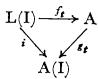
\includegraphics[keepaspectratio]{images/part001_16682a88.jpg}}

where \(i\) is the canonical injection, \(f_{t}\) is the Lie algebra homomorphism defined by \(\pmb{t}\) and \(g_{t}\) is the unital algebra homomorphism such that \(g_{t}(i) = t_{i}\) for \(i\in I\) . The diagram is commutative for \(g_{t}\circ i\) and \(f_{t}\) coincide on I. It follows that if \(\mathrm{P}\in \mathrm{L}(\mathrm{I})\) , the element \(\mathrm{P}((t_i)_{i\in I})\) defined in §2, no. 4, coincides with the element \(\mathrm{P}((t_i)_{i\in I})\) defined in Algebra, Chapter III, §2, no. 8, Example 2.

\subsection{\texorpdfstring{PROJECTOR OF \(A^{+}(\mathrm{X})\) ONTO \(\mathrm{L}(\mathrm{X})\)}{PROJECTOR OF A+ (X) ONTO L(X)}}

Let \(\pi\) be the linear mapping of \(A^{+}(X)\) into \(L(X)\) defined by

\[
\pi (x _ {1} \dots x _ {n}) = (\mathrm{ad} (x _ {1}) \circ \dots \circ \mathrm{ad} (x _ {n - 1})) (x _ {n})\tag{3}
\]

for \(n \geqslant 1, x_1, \ldots, x_n\) in X.

PROPOSITION 1. (a) The restriction \(\pi_0\) of \(\pi\) to \(\mathrm{L}(\mathbf{X})\) is a derivation of \(\mathrm{L}(\mathbf{X})\) .

\begin{enumerate}
\def\labelenumi{(\alph{enumi})}
\setcounter{enumi}{1}
\item
  For every integer \(n \geqslant 1\) and all \(u\) in \(\mathbf{L}^n(\mathbf{X})\) , \(\pi(\mathbf{u}) = n.u.\)
\item
  Let E be the endomorphism algebra of the module L(X) and \(\theta\) the homomorphism of A(X) into E such that \(\theta(x) = \operatorname{ad} x\) for all \(x \in X\) . The restriction of \(\theta\) to L(X) is a Lie algebra homomorphism of L(X) into E, which coincides on X with the adjoint representation of L(X), whence
\end{enumerate}

\[
\theta (u). v = [ u, v ] \quad \text { for   } u, v \text {   in   } L (X).\tag{4}
\]

Let \(a\) be in \(\mathrm{A}(\mathrm{X})\) and \(b\) in \(\mathrm{A}^{+}(\mathrm{X})\) ; then

\[
\pi (a. b) = \theta (a). \pi (b).\tag{5}
\]

It suffices to consider the case \(a = x_{1} \ldots x_{p}\) , \(b = x_{p+1} \ldots x_{p+q}\) with \(p \geqslant 0\) , \(q \geqslant 1\) and \(x_{1}, \ldots, x_{p+q}\) in \(\mathbf{X}\) ; but then (5) follows immediately from (3) since \(\theta(x) = \operatorname{ad} x\) for \(x \in \mathbf{X}\) .

Let \(u\) and \(v\) be in \(\mathbf{L}(\mathbf{X})\) ; by (4) and (5),

\[
\begin{array}{r l} \pi_ {0} ([ u, v ]) & = \pi (u v - v u) = \theta (u). \pi (v) - \theta (v). \pi (u) \\ & = [ u, \pi (v) ] - [ v, \pi (u) ] = [ u, \pi_ {0} (v) ] + [ \pi_ {0} (u), v ], \end{array}
\]

hence \(\pi_0\) is a derivation of L(X).

\begin{enumerate}
\def\labelenumi{(\alph{enumi})}
\setcounter{enumi}{1}
\tightlist
\item
  Let \(\pi_1\) be the endomorphism of the module \(\mathrm{L}(\mathbf{X})\) which coincides on \(\mathrm{L}^n (\mathbf{X})\) with multiplication by the integer \(n\geqslant 1\) . The formula \([\mathrm{L}^n (\mathbf{X}),\mathrm{L}^m (\mathbf{X})]\subset \mathrm{L}^{n + m}(\mathrm{X})\) shows that \(\pi_{1}\) is a derivation (Algebra, Chapter III, § 10, no. 3, Example 6). The derivation \(\pi_1 - \pi_0\) of \(\mathrm{L}(\mathbf{X})\) is zero on \(\mathbf{X}\) and, as \(\mathbf{X}\) generates \(\mathrm{L}(\mathbf{X}),\pi_0 = \pi_1\) , whence (b).
\end{enumerate}

COROLLARY. Suppose that K is a Q-algebra. Let P be the linear mapping of \(A^{+}(X)\) into itself such that

\[
\mathrm{P} \left(x _ {1} \dots x _ {n}\right) = \frac {1}{n} (\operatorname{ad} x _ {1} \circ \dots \circ \operatorname{ad} x _ {n - 1}) (x _ {n})\tag{6}
\]

for \(n \geqslant 1\) and \(x_1, \ldots, x_n\) in \(\mathbf{X}\) . Then \(\mathbf{P}\) is a projector of \(\mathbf{A}^+(\mathbf{X})\) onto \(\mathbf{L}(\mathbf{X})\) .

The image of \(\mathbf{P}\) is contained in \(\mathrm{L}(\mathrm{X})\) . Further, for all \(n \geqslant 1\) and all \(u\) in \(\mathrm{L}^n (\mathrm{X})\) , \(\mathrm{P}(u) = \frac{1}{n}\pi (u)\) , whence \(\mathrm{P}(u) = u\) by Proposition 1. As

\[
\mathrm{L} (\mathrm{X}) = \sum_ {n \geqslant 1} \mathrm{L} ^ {n} (\mathrm{X}),
\]

we see that the restriction of P to L(X) is the identity.

Remark. Suppose that K is a field of characteristic zero and let Q be the projector of A(X) = U(L(X)) onto L(X) associated with the canonical graduation of U(L(X)), cf.~§ 1, no. 5. For \(\alpha \in \mathbf{N}^{(\mathbf{X})}\) , Q(A \(^\alpha\) (X)) ⊂ L \(^\alpha\) (X). For it suffices to verify that the image and the kernel of Q are graded submodules of A(X) with the graduation of type N \(^\alpha\) . This is obvious for the image, which is equal to L(X). On the other hand, let n be an integer \(\geqslant\) 1. The vector subspace of A(X) generated by the \(y^n\) , where \(y \in L\) (X), is equal to the vector subspace of A(X) generated by the \(\sum_{\sigma \in \mathcal{E}_n} y_{\sigma(1)} y_{\sigma(2)} \ldots y_{\sigma(n)}\) , where \(y_1, y_2, \ldots, y_n\) are homogeneous elements of L(X); then this subspace is a graded submodule of A(X).

(Note that, if \(\operatorname{Card}(\mathbf{X}) \geqslant 2\) , the projectors \(\mathbf{P}\) and \(\mathbf{Q}\) do not coincide on \(\mathbf{A}^{+}(\mathbf{X})\) . For let \(x, y\) be in \(\mathbf{X}\) with \(x \neq y\) and write

\[
z = x [ x, y ] + [ x, y ] x = x ^ {2} y - y x ^ {2}.
\]

Then \(\mathbf{Q}(z) = 0\) and \(\mathrm{P}(z) = \frac{1}{3}[x, [x,y]] \neq 0\) , cf.~§2, no. 10, Example and no. 11, Theorem 1.)

\subsection{DIMENSION OF THE HOMOGENEOUS COMPONENTS OF L(X)}

Let X be a set, \(\alpha\) an element of \(\mathbf{N}^{(X)}\) and d an integer >0. We write \(d|\alpha\) if there exists \(\beta\in\mathbf{N}^{(X)}\) such that \(\alpha=d\beta\) . The element \(\beta\) , which is unique, is then denoted by \(\alpha/d\) .

Lemma 1. Let \(n\) be an integer \(>0\) , \(T_1, \ldots, T_n\) indeterminates and \(u_1, \ldots, u_n\) elements of \(\mathbf{Z}\) . Let \((c(\alpha))_{\alpha \in \mathbf{N}^n - \{0\}}\) be a family of elements of \(\mathbf{Z}\) such that

\[
1 - \sum_ {i = 1} ^ {n} u _ {i} T _ {i} = \prod_ {\alpha \neq 0} (1 - T ^ {\alpha}) ^ {c (\alpha)}.\tag{7}
\]

For all \(\alpha \in \mathbf{N}^n - \{0\}\) ,

\[
c (\alpha) = \frac {1}{| \alpha |} \sum_ {d | \alpha} \mu (d) \frac {(| \alpha | / d) !}{(\alpha / d) !} u ^ {\alpha / d}\tag{8}
\]

where \(\mu\) is the Möbius function (Appendix).

Formula (7) is equivalent, on taking logarithms on both sides (Algebra, Chapter IV, § 6, no. 9) to:

\[
\log \left(1 - \sum_ {i = 1} ^ {n} u _ {i} T _ {i}\right) = \sum_ {\alpha \neq 0} c (\alpha) \log (1 - T ^ {\alpha}).\tag{9}
\]

Now

\[
\begin{array}{r l} - \log \left(1 - \sum_ {i = 1} ^ {n} u _ {i} \mathrm{T} _ {i}\right) & = \sum_ {j \geqslant 1} \frac {1}{j} \left(\sum_ {i = 1} ^ {n} u _ {i} \mathrm{T} _ {i}\right) ^ {j} \\ & = \sum_ {j \geqslant 1} \frac {1}{j} \sum_ {| \beta | = j} \frac {| \beta | !}{\beta !} u ^ {\beta} \mathrm{T} ^ {\beta} \\ & = \sum_ {| \beta | > 0} \frac {1}{| \beta |} \frac {| \beta | !}{\beta !} u ^ {\beta} \mathrm{T} ^ {\beta}. \end{array}\tag{10}
\]

On the other hand

\[
\begin{array}{r l} - \sum_ {\alpha \neq 0} c (\alpha) \log (1 - T ^ {\alpha}) & = \sum_ {| \alpha | > 0, k \geqslant 1} \frac {1}{k} c (\alpha) T ^ {k \alpha} \\ & = \sum_ {| \beta | > 0, k | \beta} \frac {1}{k} c \left(\frac {\beta}{k}\right) T ^ {\beta}. \end{array}\tag{11}
\]

Hence (7) is equivalent to

\[
\sum_ {k \mid \beta} \left| \frac {\beta}{k} \right| c \left(\frac {\beta}{k}\right) = \frac {| \beta | !}{\beta !} u ^ {\beta} \quad \text { for   all } \beta \in \mathbf {N} ^ {n} - \{0 \}.\tag{12}
\]

Let \(\Lambda\) be the set of \((\lambda_1, \lambda_2, \ldots, \lambda_n) \in \mathbf{N}^n - \{0\}\) such that the g.c.d. of \(\lambda_1, \lambda_2, \ldots, \lambda_n\) is equal to 1. Every element of \(\mathbf{N}^n - \{0\}\) can be written uniquely

in the form \(m\lambda\) , where \(m\) is an integer \(\geqslant 1\) and \(\lambda \in \Lambda\) . Condition (12) is equivalent to

\[
\sum_ {k \mid m} \left| \frac {m \lambda}{k} \right| c \left(\frac {m \lambda}{k}\right) = \frac {(m | \lambda |) !}{(m \lambda) !} u ^ {m \lambda} \quad \text { for   all } \lambda \in \Lambda \text { and   all } m \geqslant 1.\tag{13}
\]

By the Möbius inversion formula (Appendix), condition (13) is equivalent to

\[
\left| m \lambda \right| c (m \lambda) = \sum_ {d \mid m} \mu (d) \frac {\left| \frac {m \lambda}{d} \right| !}{\left(\frac {m \lambda}{d}\right) !} u ^ {\frac {m \lambda}{d}}\tag{14}
\]

for all \(\lambda\in\Lambda\) and all \(m\geqslant1\) .

THEOREM 2. Let X be a finite set and \(n = \operatorname{Card}(X)\) .

\begin{enumerate}
\def\labelenumi{(\alph{enumi})}
\tightlist
\item
  For every integer \(r \geqslant 1\) , the K-module \(\mathbf{L}^r(\mathbf{X})\) is free of rank
\end{enumerate}

\[
c (r) = \frac {1}{r} \sum_ {d | r} \mu (d) n ^ {r / d},\tag{15}
\]

where μ is the Möbius function.

\begin{enumerate}
\def\labelenumi{(\alph{enumi})}
\setcounter{enumi}{1}
\tightlist
\item
  For all \(\alpha \in \mathbf{N}^{(\mathbf{X})} - \{0\}\) , the K-module \(\mathbf{L}^{\alpha}(\mathbf{X})\) ( \(\S 2\) , no. 6) is free of rank
\end{enumerate}

\[
c (\alpha) = \frac {1}{| \alpha |} \sum_ {d | \alpha} \mu (d) \frac {(| \alpha | / d) !}{(\alpha / d) !}.\tag{16}
\]

We already know that the modules \(L^{r}(\mathbf{X})\) , where \(r \in \mathbf{N}\) , and \(L^{\alpha}(\mathbf{X})\) , where \(\alpha \in \mathbf{N}^{\mathbf{X}}\) , are free (§ 2, no. 11, Corollary to Theorem 1). Consider the multigraduation \((A^{\alpha}(X))_{\alpha \in \mathbf{N}^{\mathbf{X}}}\) of A(X) defined by the canonical homomorphism \(\phi\) of Mo(X) into \(\mathbf{N}^{\mathbf{X}}\) (Algebra, Chapter III, § 3, no. 1, Example 3); then \(A^{\alpha}(\mathbf{X}) \cap L(\mathbf{X}) = L^{\alpha}(\mathbf{X})\) by Remark 3 of no. 1. For \(\alpha \in \mathbf{N}^{\mathbf{X}}\) , the K-module \(A^{\alpha}(\mathbf{X})\) admits as basis the set of words in which each letter \(x\) of X appears \(\alpha(x)\) times. Let \(d(\alpha)\) be the number of these words, that is the rank of \(A^{\alpha}(\mathbf{X})\) ; we shall calculate in two different ways the formal power series

defined by

\[
\mathbf {P} ((\mathrm{T} _ {x}) _ {x \in \mathbf {X}}) \in \mathbf {Z} [ [ (\mathrm{T} _ {x}) _ {x \in \mathbf {X}} ] ]\tag{17}
\]

\[
\mathrm{P} (\mathrm{T}) = \sum_ {\alpha \in \mathbf {N} ^ {\mathbf {X}}} d (\alpha) \mathrm{T} ^ {\alpha}.
\]

\begin{enumerate}
\def\labelenumi{(\arabic{enumi})}
\tightlist
\item
  We have
\end{enumerate}

\[
\mathrm{P} (\mathrm{T}) = \sum_ {m \in \mathrm{Mo} (\mathrm{X})} \mathrm{T} ^ {\phi (m)} = \sum_ {r = 0} ^ {\infty} \sum_ {x _ {1}, \dots , x _ {r}} \mathrm{T} _ {x _ {1}} \dots \mathrm{T} _ {x _ {r}} = \sum_ {r = 0} ^ {\infty} \left(\sum_ {x \in \mathrm{X}} \mathrm{T} _ {x}\right) ^ {r}
\]

whence

\[
\mathrm{P} (\mathrm{T}) = \left(1 - \sum_ {x \in \mathbf {X}} \mathrm{T} _ {x}\right) ^ {- 1}.\tag{18}
\]

\begin{enumerate}
\def\labelenumi{(\arabic{enumi})}
\setcounter{enumi}{1}
\tightlist
\item
  For all \(\alpha \in \mathbf{N}^{\mathbf{X}} - \{0\}\) , let \((e_{\alpha,j})_{1 \leqslant j \leqslant c(\alpha)}\) be a basis of \(\mathrm{L}^{\alpha}(\mathbf{X})\) and give the set I of ordered pairs \((\alpha, j)\) such that \(\alpha \in \mathbf{N}^{\mathbf{X}} - \{0\}\) and \(1 \leqslant j \leqslant c(\alpha)\) a total ordering. By Theorem 1 of no. 1 and the Poincaré-Birkhoff-Witt Theorem (Chapter I, §2, no. 7, Corollary 3 to Theorem 1), the elements
\end{enumerate}

\[
y _ {m} = \prod_ {(\alpha , j) \in \mathbb {I}} (e _ {\alpha , j}) ^ {m (\alpha , j)},
\]

where the index \(\pmb{m}\) runs through \(\mathbf{N}^{(I)}\) , form a basis of \(A(\mathbf{X})\) . Each \(y_{m}\) is of a multidegree \(\sum_{(\alpha, j) \in I} \pmb{m}(\alpha, j)\alpha\) . Let \(u(\pmb{m})\) denote this multidegree. It follows that

\[
\begin{array}{l} \mathrm{P(T)} = \sum_ {m \in \mathrm{N} ^ {(I)}} \mathrm{T} ^ {u (m)} = \sum_ {m \in \mathrm{N} ^ {(I)}} \prod_ {(\alpha , j) \in I} \mathrm{T} ^ {m (\alpha , j) \alpha} \\ = \prod_ {(\alpha , j) \in I} \sum_ {r = 0} ^ {\infty} \mathrm{T} ^ {r \alpha} = \prod_ {(\alpha , j) \in I} (1 - \mathrm{T} ^ {\alpha}) ^ {- 1}, \end{array}
\]

whence finally

\[
\mathrm{P} (\mathrm{T}) = \prod_ {\alpha \in \mathbf {N} ^ {\mathbf {X}} - \{0 \}} (1 - \mathrm{T} ^ {\alpha}) ^ {- c (\alpha)}.\tag{19}
\]

Comparing (18) and (19), we obtain

\[
1 - \sum_ {x \in \mathbf {X}} T _ {x} = \prod_ {\alpha \in \mathbf {N} ^ {\mathbf {X}} - \{0\}} (1 - T ^ {\alpha}) ^ {c (\alpha)}.\tag{20}
\]

Lemma 1 then gives (b).

If we now substitute the same indeterminate U for the \(T_{x}\) for \(x \in X\) in formula (20), we obtain

\[
1 - n \mathrm{U} = \prod_ {\alpha \in \mathbf {N} ^ {\mathrm{X}} - \{0\}} (1 - \mathrm{U} ^ {| \alpha |}) ^ {c (\alpha)} = \prod_ {r > 0} (1 - \mathrm{U} ^ {r}) ^ {c (r)}.
\]

Applying Lemma 1 again, we deduce (a).

Examples. We have

\[
\begin{array}{l l} c (1) = n, & c (2) = \frac {1}{2} (n ^ {2} - n), \qquad c (3) = \frac {1}{3} (n ^ {3} - n), \\ c (4) = \frac {1}{4} (n ^ {4} - n ^ {2}), & c (5) = \frac {1}{5} (n ^ {5} - n), \qquad c (6) = \frac {1}{6} (n ^ {6} - n ^ {3} - n ^ {2} + n). \end{array}
\]

Remark. Let X be a set and let \(\alpha \in \mathbf{N}^{(X)}\) ; the rank of the free K-module \(\mathbf{L}^{\alpha}(X)\) is also given by formula (16). This follows immediately from Theorem 2 (b) and Proposition 4 of § 2, no. 6.

\section{CENTRAL FILTRATIONS}

\subsection{REAL FILTRATIONS}

DEFINITION 1. Let G be a group. A real filtration on G is a family \((\mathrm{G}_{\alpha})_{\alpha \in \mathbf{R}}\) of subgroups of G such that

\[
\mathrm{G} _ {\alpha} = \bigcap_ {\beta <   \alpha} \mathrm{G} _ {\beta} \text {   for   all   } \alpha \in \mathbf {R}.\tag{1}
\]

Formula (1) implies \(G_{\alpha} \subset G_{\beta}\) for \(\beta < \alpha\) and hence the family \((\mathrm{G}_{\alpha})\) is decreasing. The filtration \((\mathrm{G}_{\alpha})\) is called separated if \(\bigcap_{\alpha} G_{\alpha}\) reduces to the identity element and is called exhaustive if \(G = \bigcup_{\alpha} G_{\alpha}\) .

Remark. Let \((\mathrm{G}_n)_{n\in \mathbf{Z}}\) be a decreasing sequence of subgroups of G. It is a decreasing filtration in the sense of Commutative Algebra, Chapter III, § 2, no. 1, Definition 1. For every integer \(n\) and all \(\alpha\) in the interval \(]n - 1,n]\) of \(\mathbf{R}\) , we write \(\mathrm{H}_{\alpha} = \mathrm{G}_{n}\) , in particular \(\mathrm{H}_n = \mathrm{G}_n\) . It is immediate that we thus obtain a real filtration \((\mathrm{H}_{\alpha})_{\alpha \in \mathbf{R}}\) on G; such a filtration will be called an integral filtration. Hence decreasing filtrations in the sense of Commutative Algebra, Chapter III, § 2, can be identified with integral filtrations.

Let A be an algebra; a real filtration \((\mathrm{A}_{\alpha})\) on the additive group of A is called compatible with the algebra structure if \(\mathrm{A}_{\alpha}.\mathrm{A}_{\beta}\subset \mathrm{A}_{\alpha +\beta}\) for \(\alpha ,\beta\) in R and \(\mathrm{K.A}_{\alpha}\subset \mathrm{A}_{\alpha}\) for \(\alpha \in \mathbf{R}\) . If the filtration is exhaustive, \((\mathrm{A}_{\alpha})\) is a fundamental system of neighbourhoods of 0 under the topology on A which is compatible with the algebra structure. Let B be a unital algebra; a real filtration \((\mathrm{B}_{\alpha})\) on the additive group of B is called compatible with the unital algebra structure if it is compatible with the algebra structure and \(1\in \mathrm{B}_0\) .

\subsection{ORDER FUNCTION}

Let \(G\) be a group with identity element \(e\) . Let \((\mathbf{G}_{\alpha})\) be a real filtration on \(G\) . For all \(x\) in \(G\) let \(I_x\) denote the set of real numbers \(\alpha\) such that \(x \in G_{\alpha}\) . If \(\alpha \in I_x\) and \(\beta < \alpha\) , then \(\beta \in I_x\) and hence \(I_x\) is an interval (General Topology, Chapter IV, § 2, no. 4, Proposition 1). Using relation (1), we see that \(I_x\) contains its least upper bound when this is finite. Therefore \(I_x\) is of the form \(] - \infty\) , \(v(x)] \cap R\) with \(v(x) \in \overline{\mathbf{R}}\) ; we have \(v(x) = \sup(\alpha \mid x \in G_{\alpha})\) .

The mapping \(v\) of \(G\) into \(\overline{\mathbf{R}}\) is called the order function associated with the real filtration \((G_{\alpha})\) and \(v(x)\) is called the order of \(x\) . This mapping has the following properties:

\begin{enumerate}
\def\labelenumi{(\alph{enumi})}
\item
  For \(x \in \mathbf{G}\) and \(\alpha \in \mathbf{R}\) , the relations \(x \in \mathbf{G}_{\alpha}\) and \(v(x) \geqslant \alpha\) are equivalent.
\item
  For x, y in G,
\end{enumerate}

\begin{enumerate}
\def\labelenumi{(\arabic{enumi})}
\setcounter{enumi}{1}
\tightlist
\item
\end{enumerate}

\[
v (x ^ {- 1}) = v (x), \quad v (e) = + \infty .\tag{2}
\]

\[
v (x y) \geqslant \inf (v (x), v (y)).\tag{3}
\]

Further, we have equality in (3) if \(v(x) > v(y)\) .

\begin{enumerate}
\def\labelenumi{(\alph{enumi})}
\setcounter{enumi}{2}
\tightlist
\item
  For all \(\alpha \in \mathbf{R}\) , let \(\mathrm{G}_{\alpha}^{+}\) denote the set of \(x \in \mathrm{G}\) such that \(v(x) > \alpha\) . Then \(\mathrm{G}_{\alpha}^{+} = \bigcup_{\beta > \alpha} \mathrm{G}_{\beta}\) and in particular \(\mathrm{G}_{\alpha}^{+}\) is a subgroup of \(\mathrm{G}\) .
\end{enumerate}

Conversely, let \(v\) be a mapping of \(G\) into \(\overline{\mathbf{R}}\) satisfying relations (2) and (3). For all \(\alpha \in \mathbf{R}\) , let \(G_{\alpha}\) be the set of \(x \in G\) such that \(v(x) \geqslant \alpha\) . Then \((G_{\alpha})_{\alpha \in \mathbf{R}}\) is a real filtration of \(G\) and \(v\) is the order function associated with this filtration.

For the filtration \((\mathbf{G}_{\alpha})\) to be integral, it is necessary and sufficient that \(v\) map \(\mathbf{G}\) into \(\mathbf{Z} \cup \{+\infty, -\infty\}\) . For it to be exhaustive (resp. separated), it is necessary and sufficient that \(v^{-1}(-\infty) = \varnothing\) (resp. \(v^{-1}(+\infty) = \{e\}\) ).

Let A be a K-algebra (resp. unital K-algebra). By the above, the relation

\[
" x \in \mathrm{A} _ {\alpha} \Leftrightarrow v (x) \geqslant \alpha \quad \text { for } x \in \mathrm{A} \text { and } \alpha \in \mathbf {R}"
\]

defines a bijection of the set of exhaustive real filtrations \((\mathbf{A}_{\alpha})_{\alpha\in\mathbf{R}}\) compatible with the algebra (resp. unital algebra) structure on A onto the set of mappings \(v: A \to \overline{\mathbf{R}}\) not taking the value \(-\infty\) and satisfying axioms (4) to (7) (resp. (4) to (8)) below:

\begin{enumerate}
\def\labelenumi{(\arabic{enumi})}
\setcounter{enumi}{3}
\tightlist
\item
\end{enumerate}

\[
v (x + y) \geqslant \inf (v (x), v (y)) \quad (x, y \text {   in   A })\tag{5}
\]

\[
v (- x) = v (x) \quad (x \in \mathrm{A})\tag{6}
\]

\[
v (\lambda x) \geqslant v (x) \quad (\lambda \in \mathrm{K}, x \in \mathrm{A})\tag{7}
\]

\[
v (x y) \geqslant v (x) + v (y) \quad (x, y \text {   in   A })\tag{8}
\]

\[
v (1) \geqslant 0.
\]

Remark. If \(v(x)\) is not everywhere equal to \(+\infty\) , conditions (7) and (8) imply \(v(1) = 0\) .

\subsection{GRADED ALGEBRA ASSOCIATED WITH A FILTERED ALGEBRA}

Let G be a commutative group with a real filtration \((G_{\alpha})_{\alpha \in \mathbb{R}}\) . As before we write

\[
\mathrm{G} _ {\alpha} ^ {+} = \bigcup_ {\beta > \alpha} \mathrm{G} _ {\beta};\tag{9}
\]

clearly \(\mathrm{G}_{\alpha}^{+}\) is a subgroup of \(\mathrm{G}_{\alpha}\) . We write \(\mathrm{gr}_{\alpha}(\mathrm{G}) = \mathrm{G}_{\alpha} / \mathrm{G}_{\alpha}^{+}\) and

\[
\operatorname{gr} (\mathrm{G}) = \bigoplus_ {\alpha \in \mathbf {R}} \operatorname{gr} _ {\alpha} (\mathrm{G}).
\]

The graded group associated with the filtered group G is the group \(\operatorname{gr}(G)\) with its natural graduation of type R.

Remark. When the filtration \((\mathrm{G}_{\alpha})\) is integral, \(\mathrm{gr}_{\alpha}(\mathrm{G}) = \{0\}\) for non-integral \(\alpha\) and \(\mathrm{gr}_n(\mathrm{G}) = \mathrm{G}_n / \mathrm{G}_{n - 1}\) for every integer \(n\) . The definition of the associated graded group therefore coincides essentially with that of Commutative Algebra, Chapter III, § 2, no. 3.

Let \(\mathbf{A}\) be an algebra (resp. unital algebra) and \((\mathbf{A}_{\alpha})_{\alpha \in \mathbb{R}}\) a real filtration compatible with the algebra (resp. unital algebra) structure (no. 1). Then

\[
\mathrm{A} _ {\alpha}. \mathrm{A} _ {\beta} \subset \mathrm{A} _ {\alpha + \beta}, \quad \mathrm{A} _ {\alpha} ^ {+}. \mathrm{A} _ {\beta} + \mathrm{A} _ {\alpha}. \mathrm{A} _ {\beta} ^ {+} \subset \mathrm{A} _ {\alpha + \beta} ^ {+},
\]

and the bilinear mapping of \(A_{\alpha} \times A_{\beta}\) into \(A_{\alpha+\beta}\) the restriction of multiplication on A defines on taking quotients a bilinear mapping

\[
\operatorname{gr} _ {\alpha} (\mathrm{A}) \times \operatorname{gr} _ {\beta} (\mathrm{A}) \rightarrow \operatorname{gr} _ {\alpha + \beta} (\mathrm{A}).
\]

We derive a bilinear mapping of \(\mathrm{gr}(\mathbf{A}) \times \mathrm{gr}(\mathbf{A})\) into \(\mathrm{gr}(\mathbf{A})\) which makes it a graded algebra (resp. unital graded algebra) of type R. If A is an associative (resp. commutative, resp. Lie) algebra, so is \(\mathrm{gr}(\mathbf{A})\) .

\subsection{CENTRAL FILTRATIONS ON A GROUP}

DEFINITION 2. Let G be a group. A real filtration \((\mathrm{G}_{\alpha})\) on G is called central if \(\mathrm{G} = \bigcup_{\alpha >0}\mathrm{G}_{\alpha}\) and the commutator \((x,y) = x^{-1}y^{-1}xy\) of an element \(x\) of \(\mathrm{G}_{\alpha}\) and an element \(y\) of \(\mathrm{G}_{\beta}\) belongs to \(\mathrm{G}_{\alpha +\beta}\) .

In terms of the order function v, the above definition translates into the relations

\[
v (x) > 0, \quad v ((x, y)) \geqslant v (x) + v (y) \quad \text { for   all } x, y \text { in } G.\tag{10}
\]

We deduce that \(v((x,y)) > v(x)\) if \(v(x) \neq +\infty\) ; if we write \(x^y = y^{-1}xy\) (cf.~Algebra, Chapter I, § 6, no. 2), then \(x^y = x.(x,y)\) , whence

\[
v (x ^ {y}) = v (x).\tag{11}
\]

This relation expresses the fact that each of the subgroups \(G_{\alpha}\) of G is normal. The \(G_{\alpha}\) form a fundamental system of neighbourhoods of e for a topology compatible with the group structure on G (General Topology, Chapter III, § 1, no. 2, Example) said to be defined by the filtration ( \(G_{\alpha}\) ).

In the rest of this no., G denotes a group with a central filtration \((G_{\alpha})\) . For all \(\alpha \in R\) , we define the subgroup \(G_{\alpha}^{+}\) of G by

\[
\mathrm{G} _ {\alpha} ^ {+} = \bigcup_ {\beta > \alpha} \mathrm{G} _ {\beta}.\tag{12}
\]

In particular \(G_{\alpha}^{+} = G_{\alpha} = G\) for \(\alpha \leqslant 0\) . Recall that if A and B are two subgroups of G, (A, B) denotes the subgroup of G generated by the commutators \((a, b)\) with \(a \in A\) and \(b \in B\) . With this notation we have the formulae

\begin{enumerate}
\def\labelenumi{(\arabic{enumi})}
\setcounter{enumi}{12}
\tightlist
\item
\end{enumerate}

\[
\left(\mathrm{G} _ {\alpha}, \mathrm{G} _ {\beta}\right) \subset \mathrm{G} _ {\alpha + \beta}\tag{13}
\]

\[
\left(\mathrm{G} _ {\alpha} ^ {+}, \mathrm{G} _ {\beta}\right) \subset \mathrm{G} _ {\alpha + \beta} ^ {+}\tag{13'}
\]

\[
(G, G _ {\alpha}) \subset G _ {\alpha} ^ {+}.\tag{14}
\]

By (14), \(\mathrm{G}_{\alpha}^{+}\) is a normal subgroup of \(\mathrm{G}_{\alpha}\) for all \(\alpha \in \mathbf{R}\) and the quotient group \(\mathrm{gr}_{\alpha}(\mathrm{G}) = \mathrm{G}_{\alpha} / \mathrm{G}_{\alpha}^{+}\) is commutative. We write \(\mathrm{gr}(\mathrm{G}) = \bigoplus_{\alpha \in \mathbb{R}}\mathrm{gr}_{\alpha}(\mathrm{G})\) and give this group the graduation of type \(\mathbf{R}\) in which \(\mathrm{gr}_{\alpha}(\mathrm{G})\) consists of elements of degree \(\alpha\) . Then \(\mathrm{gr}_{\alpha}(\mathrm{G}) = \{0\}\) for \(\alpha \leqslant 0\) .

PROPOSITION 1. (i) Let \(\alpha, \beta\) be in \(\mathbf{R}\) . There exists a biadditive mapping

\[
\phi_ {\alpha \beta}: \operatorname{gr} _ {\alpha} (\mathrm{G}) \times \operatorname{gr} _ {\beta} (\mathrm{G}) \rightarrow \operatorname{gr} _ {\alpha + \beta} (\mathrm{G})
\]

which maps \((x\mathrm{G}_{\alpha}^{+},y\mathrm{G}_{\beta}^{+})\) onto \((x,y)\mathrm{G}_{\alpha +\beta}^{+}\)

\begin{enumerate}
\def\labelenumi{(\roman{enumi})}
\setcounter{enumi}{1}
\item
  Let \(\phi\) be the biadditive mapping of \(\operatorname{gr}(\mathbf{G}) \times \operatorname{gr}(\mathbf{G})\) into \(\operatorname{gr}(\mathbf{G})\) whose restriction to \(\operatorname{gr}_{\alpha}(\mathbf{G}) \times \operatorname{gr}_{\beta}(\mathbf{G})\) is \(\phi_{\alpha \beta}\) for every ordered pair \((\alpha, \beta)\) . The mapping \(\phi\) gives \(\operatorname{gr}(\mathbf{G})\) a Lie Z-algebra structure.
\item
  Recall the identity
\end{enumerate}

\[
(x x ^ {\prime}, y) = (x, y) ^ {x ^ {\prime}} \left(x ^ {\prime}, y\right)\tag{15}
\]

for \(x, x', y\) in \(\mathbf{G}\) (Algebra, Chapter I, § 6, no. 2, formula (4 bis)).

For \(x \in G_{\alpha}\) and \(y \in G_{\beta}\) , the class modulo \(G_{\alpha + \beta}^{+}\) of the element \((x, y)\) of \(G_{\alpha + \beta}\) will be denoted by \(f(x, y)\) . For \(a\) in \(G_{\alpha + \beta}\) and \(x'\) in \(G, a^{-1}.a^{x'} = (a, x') \in G_{\alpha + \beta}^{+}\) ; in particular \(f(x, y)\) is equal to the class modulo \(G_{\alpha + \beta}^{+}\) of \((x, y)^{x'}\) . Formula (15) therefore implies

\[
f (x x ^ {\prime}, y) = f (x, y) f (x ^ {\prime}, y).\tag{16}
\]

Now \((y, x) = (x, y)^{-1}\) , whence

\[
f (y, x) = f (x, y) ^ {- 1}.\tag{17}
\]

From (16) and (17) we deduce

\[
f (x, y y ^ {\prime}) = f (x, y) f (x, y ^ {\prime}).\tag{18}
\]

We have to prove that the mapping \(f\colon \mathrm{G}_{\alpha}\times \mathrm{G}_{\beta}\to \mathrm{gr}_{\alpha +\beta}(\mathrm{G})\) defines on taking quotients a mapping \(\phi_{\alpha \beta}\colon \mathrm{gr}_{\alpha}(\mathrm{G})\times \mathrm{gr}_{\beta}(\mathrm{G})\to \mathrm{gr}_{\alpha +\beta}(\mathrm{G})\) . By (16) and (18) it suffices to prove that \(f(x,y) = 0\) if \(x\in \mathrm{G}_{\alpha}^{+}\) or \(y\in \mathrm{G}_{\beta}^{+}\) , which follows from (13').

\begin{enumerate}
\def\labelenumi{(\roman{enumi})}
\setcounter{enumi}{1}
\tightlist
\item
  As \((x, x) = e\) , it follows from (17) that \(\phi\) is an alternating \(\mathbf{Z}\) -bilinear mapping. Hence it remains to prove that, for \(u \in \mathrm{gr}_{\alpha}(\mathrm{G})\) , \(v \in \mathrm{gr}_{\beta}(\mathrm{G})\) and \(w \in \mathrm{gr}_{\gamma}(\mathrm{G})\) ,
\end{enumerate}

\[
\phi (u, \phi (v, w)) + \phi (v, \phi (w, u)) + \phi (w, \phi (u, v)) = 0.\tag{19}
\]

Let \(x \in G_{\alpha}, y \in G_{\beta}\) and \(z \in G_{\gamma}\) be elements representing respectively \(u, v\) and \(w\) . We know that \(x^{y}\) and \(x\) are two elements of \(G_{\alpha}\) which are congruent modulo \(G_{\alpha}^{+}\) and hence \(x^{y}\) is a representative of \(u\) in \(G_{\alpha}\) ; as \((y, z)\) is a representative of \(\phi(v, w)\) in \(G_{\beta + \gamma}\) , we see that \((x^{y}, (y, z))\) is a representative of \(\phi(u, \phi(v, w))\) in \(G_{\alpha + \beta + \gamma}\) . By cyclic permutation, we see that \((y^{z}, (z, x))\) and \((z^{x}, (x, y))\) represent respectively \(\phi(v, \phi(w, u))\) and \(\phi(w, \phi(u, v))\) in \(G_{\alpha + \beta + \gamma}\) . Relation (19) is then a consequence of the following identity (Algebra, Chapter I, §6, no. 2, formula (15)):

\[
\left(x ^ {y}, (y, z)\right). \left(y ^ {z}, (z, x)\right). \left(z ^ {x}, (x, y)\right) = e.\tag{20}
\]

The Lie algebra \(\mathrm{gr}(\mathbf{G})\) over \(\mathbf{Z}\) defined in Proposition 1 is called the graded Lie algebra associated with the filtered group \(\mathbf{G}\) .

\subsection{AN EXAMPLE OF A CENTRAL FILTRATION}

Let \(\mathbf{A}\) be a unital associative algebra with a unital algebra filtration \((\mathbf{A}_{\alpha})\) such that \(\mathbf{A}_{0} = \mathbf{A}\) ; then \(\mathbf{A}_{\alpha}\) is a two-sided ideal of \(\mathbf{A}\) for all \(\alpha \in \mathbf{R}\) . Let \(\mathbf{A}^*\) denote the multiplicative group of invertible elements of \(\mathbf{A}\) . For all \(\alpha > 0\) , let \(\Gamma_{\alpha}\) denote the set of \(x \in \mathbf{A}^*\) such that \(x - 1 \in \mathbf{A}_{\alpha}\) ; we write \(\Gamma = \bigcup_{\alpha > 0} \Gamma_{\alpha}\) and \(\Gamma_{\beta} = \Gamma\) for \(\beta \leqslant 0\) .

PROPOSITION 2. The set \(\Gamma\) is a subgroup of \(\mathbf{A}^*\) and \((\Gamma_{\alpha})\) is a central filtration on \(\Gamma\) .

\(\Gamma = \bigcup_{\alpha > 0} \Gamma_{\alpha}\) by construction and the relation \(\Gamma_{\alpha} = \bigcap_{\beta < \alpha} \Gamma_{\beta}\) follows from \(A_{\alpha} = \bigcap_{\beta < \alpha} A_{\beta}\) .

We show that \(\Gamma_{\alpha}\) is a subgroup of \(\mathbf{A}^*\) . Now \(1 \in \Gamma_{\alpha}\) ; let \(x, y\) be in \(\Gamma_{\alpha}\) , whence \(x - 1 \in \mathbf{A}_{\alpha}, y - 1 \in \mathbf{A}_{\alpha}\) . As \(\mathbf{A}_{\alpha}\) is a two-sided ideal of \(\mathbf{A}\) , the formulae

\begin{enumerate}
\def\labelenumi{(\arabic{enumi})}
\setcounter{enumi}{20}
\tightlist
\item
\end{enumerate}

\[
x y - 1 = (x - 1) (y - 1) + (x - 1) + (y - 1),\tag{21}
\]

\[
x ^ {- 1} - 1 = - x ^ {- 1} (x - 1),\tag{22}
\]

imply \(xy - 1 \in A_{\alpha}\) and \(x^{-1} - 1 \in A_{\alpha}\) , whence \(xy \in \Gamma_{\alpha}\) and \(x^{-1} \in \Gamma_{\alpha}\) .

As \(\Gamma = \bigcup_{\alpha > 0} \Gamma_{\alpha}\) , this is a subgroup of \(A^{*}\) .

Finally let \(\alpha > 0, \beta > 0, x \in \Gamma_{\alpha}\) and \(y \in \Gamma_{\beta}\) . Let \(x - 1 = \xi\) and \(y - 1 = \eta\) . Then

\[
(x, y) - 1 = x ^ {- 1} y ^ {- 1} (\xi \eta - \eta \xi);\tag{23}
\]

by hypothesis, \(\xi \in \mathbf{A}_{\alpha}\) and \(\eta \in \mathbf{A}_{\beta}\) , whence \(\xi \eta - \eta \xi \in \mathbf{A}_{\alpha + \beta}\) . As \(\mathbf{A}_{\alpha + \beta}\) is a two-sided ideal of \(\mathbf{A}, (x, y) - 1 \in \mathbf{A}_{\alpha + \beta}\) , whence \((x, y) \in \Gamma_{\alpha + \beta}\) .

Remark. Let \(\alpha \geqslant 0, \beta \geqslant 0\) and \(x \in \Gamma_{\alpha}, y \in \Gamma_{\beta}\) . By formulae (21), (22) and (23),

\begin{enumerate}
\def\labelenumi{(\arabic{enumi})}
\setcounter{enumi}{23}
\tightlist
\item
\end{enumerate}

\[
x ^ {- 1} - 1 \equiv - (x - 1) \quad \text { mod. } A _ {2 \alpha}\tag{24}
\]

\[
x y - 1 \equiv (x - 1) + (y - 1) \quad \text { mod. } A _ {\alpha + \beta}\tag{25}
\]

\[
(x, y) - 1 \equiv [ (x - 1), (y - 1) ] \mod A _ {\alpha + \beta + \inf (\alpha , \beta)}.\tag{26}
\]

We prove for example (26). If \(x - 1 = \xi\) and \(y - 1 = \eta\) , (23) gives:

\[
(x, y) - 1 - [ \xi , \eta ] = ((x ^ {- 1} - 1) + (y ^ {- 1} - 1) + (x ^ {- 1} - 1) (y ^ {- 1} - 1)) [ \xi , \eta ].
\]

Now \([\xi, \eta] \in \mathrm{A}_{\alpha + \beta}, (x^{-1} - 1) \in \mathrm{A}_{\alpha}, (y^{-1} - 1) \in \mathrm{A}_{\beta}\) , whence we obtain (26).

Let \(G\) be a group and \(\rho: G \to \Gamma\) a homomorphism. For all real \(\alpha\) , we write \(G_{\alpha} = \rho^{-1}(\Gamma_{\alpha})\) . As \((\Gamma_{\alpha})\) is a central filtration on \(\Gamma\) , it is immediate that \((G_{\alpha})\) is a central filtration on \(G\) .

PROPOSITION 3. (i) For all \(\alpha \in \mathbf{R}\) , there exists a unique group homomorphism \(g_{\alpha} \colon \mathrm{gr}_{\alpha}(\mathrm{G}) \to \mathrm{gr}_{\alpha}(\mathrm{A})\) which maps the class modulo \(\mathrm{G}_{\alpha}^{+}\) of an element \(a \in \mathrm{G}_{\alpha}\) to the class modulo \(\mathrm{A}_{\alpha}^{+}\) of \(\rho(a) - 1\) .

\begin{enumerate}
\def\labelenumi{(\roman{enumi})}
\setcounter{enumi}{1}
\item
  Let \(g\) be the group homomorphism of \(\mathrm{gr}(\mathrm{G})\) into \(\mathrm{gr}(\mathrm{A})\) whose restriction to \(\mathrm{gr}_{\alpha}(\mathrm{G})\) is \(g_{\alpha}\) for all \(\alpha\) . The mapping \(g\) is an injective homomorphism of Lie Z-algebras. (i) Let \(\alpha > 0\) . By hypothesis, for all \(a\) in \(\mathrm{G}_{\alpha}, \rho(a) - 1 \in \mathrm{A}_{\alpha}\) ; let \(p_{\alpha}(a)\) denote the class of \(\rho(a) - 1\) modulo \(\mathrm{A}_{\alpha}^{+}\) . As \(\mathrm{A}_{\alpha} \subset \mathrm{A}_{\alpha}^{+}\) , relation (25) implies \(p_{\alpha}(ab) = p_{\alpha}(a) + p_{\alpha}(b)\) . Then \(a \in \mathrm{G}_{\alpha}^{+}\) if and only if \(\rho(a) - 1 \in \mathrm{A}_{\alpha}^{+}\) ; therefore \(\mathrm{G}_{\alpha}^{+}\) is the kernel of the homomorphism \(p_{\alpha}\) of \(\mathrm{G}_{\alpha}\) into \(\mathrm{gr}_{\alpha}(\mathrm{A})\) . On passing to the quotient, \(p_{\alpha}\) then defines an injective homomorphism \(g_{\alpha}\) of \(\mathrm{gr}_{\alpha}(\mathrm{G})\) into \(\mathrm{gr}_{\alpha}(\mathrm{A})\) . For \(\alpha \leqslant 0\) , \(\mathrm{gr}_{\alpha}(\mathrm{G}) = \{0\}\) and the only choice is \(g_{\alpha} = 0\) .
\item
  As \(g_{\alpha}\) is injective for all real \(\alpha\) , \(g\) is injective. We show that \(g\) is a Lie algebra homomorphism. As \(\mathrm{gr}_{\alpha}(\mathrm{G}) = \{0\}\) for \(\alpha \leqslant 0\) , it suffices to establish the formula
\end{enumerate}

\[
p _ {\alpha + \beta} ((a, b)) = [ p _ {\alpha} (a), p _ {\beta} (b) ]\tag{27}
\]

for \(\alpha > 0\) , \(\beta > 0\) , \(a \in G_{\alpha}\) and \(b \in G_{\beta}\) , which follows from (26).

\subsection{INTEGRAL CENTRAL FILTRATIONS}

Recall (no. 1, Remark) that a filtration \((\mathrm{G}_{\alpha})\) on the group G is called integral if \(\mathrm{G}_{\alpha} = \mathrm{G}_{n}\) for every integer \(n\) and all \(\alpha \in ]n - 1,n]\) . To be given an integral central filtration on a group G is equivalent to being given a sequence \((\mathrm{G}_n)_{n\geqslant 1}\) of subgroups of G satisfying the conditions

\begin{enumerate}
\def\labelenumi{(\roman{enumi})}
\tightlist
\item
\end{enumerate}

\[
\mathrm{G} _ {1} = \mathrm{G}\tag{i}
\]

\[
\mathrm{G} _ {n} \supset \mathrm{G} _ {n + 1} \quad \text { for   all } n \geqslant 1\tag{ii}
\]

\[
\left(\mathrm{G} _ {m}, \mathrm{G} _ {n}\right) \subset \mathrm{G} _ {m + n} \quad \text { for } m \geqslant 1 \text { and } n \geqslant 1.\tag{iii}
\]

For every integer \(n \geqslant 1\) , \(G_n\) is a normal subgroup of \(G\) and the quotient \(\mathrm{gr}_n(G) = G_n / G_{n+1}\) is commutative. On taking quotients, the mapping \((x,y) \mapsto (x,y) = x^{-1}y^{-1}xy\) of \(G_m \times G_n\) into \(G_{m+n}\) allows us to define on \(\mathrm{gr}(G) = \bigoplus_{n \geqslant 1} \mathrm{gr}_n(G)\) a graded Lie algebra structure of type \(N\) over the ring \(Z\) .

Recall (Algebra, Chapter I, §6, no. 3, Definition 5) that the lower central series of the group \(\mathbf{G}\) is defined by

\[
\mathrm{C} ^ {1} \mathrm{G} = \mathrm{G}, \quad \mathrm{C} ^ {n + 1} = (\mathrm{G}, \mathrm{C} ^ {n} \mathrm{G}) \quad \text { for } n \geqslant 1.\tag{28}
\]

The corresponding filtration is called the lower central filtration of G.

PROPOSITION 4. (i) The lower central series of G is an integral central filtration on G.

\begin{enumerate}
\def\labelenumi{(\roman{enumi})}
\setcounter{enumi}{1}
\tightlist
\item
  If \((\mathrm{G}_n)_{n\in \mathbf{N}^*}\) is an integral central filtration on \(\mathbf{G}\) , then \(\mathbf{C}^n\mathbf{G}\subset \mathbf{G}_n\) for all \(n\in \mathbf{N}^*\) .
\end{enumerate}

Assertion (i) has been proved in Algebra, Chapter I, § 6, no. 3, formula (7).

We prove (ii) by induction on \(n\) ; \(\mathrm{C}^1\mathrm{G} = \mathrm{G} = \mathrm{G}_1\) ; for \(n > 1\) ,

\[
\mathrm{C} ^ {n} \mathrm{G} = (\mathrm{G}, \mathrm{C} ^ {n - 1} \mathrm{G}) \subset (\mathrm{G}, \mathrm{G} _ {n - 1}) \subset \mathrm{G} _ {n}.
\]

PROPOSITION 5. Let \(\mathbf{G}\) be a group and \(\operatorname{gr}(\mathbf{G})\) the graded Lie \(\mathbf{Z}\) -algebra associated with the lower central filtration on \(\mathbf{G}\) . Then \(\operatorname{gr}(\mathbf{G})\) is generated by \(\operatorname{gr}_1(\mathbf{G}) = \mathbf{G}/(\mathbf{G},\mathbf{G})\) .

Let L be the Lie subalgebra of \(\mathrm{gr}(\mathrm{G})\) generated by \(\mathrm{gr}_{1}(\mathrm{G})\) ; we show that \(\mathrm{L} \supset \mathrm{gr}_{n}(\mathrm{G})\) by induction on n, the assertion being trivial for n = 1. Suppose that n > 1 and \(\mathrm{L} \supset \mathrm{gr}_{n-1}(\mathrm{G})\) . As \(\mathrm{C}^{n}\mathrm{G} = (\mathrm{G}, \mathrm{C}^{n-1}\mathrm{G})\) , the construction of the Lie algebra law on \(\mathrm{gr}(\mathrm{G})\) shows immediately that

\[
\operatorname{gr} _ {n} (\mathrm{G}) = \left[ \operatorname{gr} _ {1} (\mathrm{G}), \operatorname{gr} _ {n - 1} (\mathrm{G}) \right] \subset \mathrm{L}.
\]

The above proof shows that the lower central series of the Lie algebra \(\mathbf{gr}(\mathbf{G})\) (§ 2, no. 7) is given by

\[
\mathcal {C} ^ {n} (\mathrm{gr} (G)) = \sum_ {m \geqslant n} \mathrm{gr} _ {m} (G).\tag{29}
\]

Remark. Let \(k\) be a ring, \(n\) an integer \(>0\) and A set of lower triangular matrices with \(n\) rows and \(n\) columns and elements in \(k\) . For \(p \geqslant 0\) , let \(\mathbf{A}_p\) be the set of \((x_{ij}) \in \mathbb{A}\) such that \(x_{ij} = 0\) for \(i - j < p\) . Then \(\mathrm{A}_0 = \mathrm{A}\) and \(\mathrm{A}_p\mathrm{A}_q \subset \mathrm{A}_{p + q}\) . Let \(\Gamma_p = 1 + \mathrm{A}_p\) . Then \(\Gamma_1\) is a subgroup of \(\mathbf{GL}(n,k)\) called the strict lower triangular group of order \(n\) over \(k\) . By Proposition 2 of no. 5, \((\Gamma_p)\) is an integral filtration on \(\Gamma_1\) . As \(\Gamma_n = \{1\}\) , we see that the group \(\Gamma_1\) is nilpotent (Algebra, Chapter I, §6, no. 3, Definition 6).

\section{MAGNUS ALGEBRAS}

In this paragraph, X denotes a set, F(X) the free group constructed on X (Algebra, Chapter I, § 7, no. 5) and A(X) the free associative algebra constructed on X with its total graduation (A \(^{n}\) (X)) \(_{n\geqslant0}\) (cf.~Algebra, Chapter III, § 3, no. 1, Example 3). X is identified with its images in F(X) and A(X).

\subsection{MAGNUS ALGEBRAS}

Let \(\hat{\mathbf{A}}(\mathbf{X})\) be the product module \(\prod_{n\geqslant 0}\mathbf{A}^n (\mathbf{X})\) . We define on \(\hat{\mathbf{A}}(\mathbf{X})\) a multiplication by the rule

\[
(a. b) _ {n} = \sum_ {i = 0} ^ {n} a _ {i}. b _ {n - i}\tag{1}
\]

where \(a = (a_{n})\) and \(b = (b_{n})\) are in \(\hat{\mathbf{A}}(\mathbf{X})\) . We know (Commutative Algebra, Chapter III, §2, no. 12, Example 1) that \(\hat{\mathbf{A}}(\mathbf{X})\) is an associative algebra and that \(\mathbf{A}(\mathbf{X})\) is identified with the subalgebra of \(\hat{\mathbf{A}}(\mathbf{X})\) consisting of the sequence all of whose terms are zero except for a finite number.

\(\hat{A}(X)\) is given the product topology of the discrete topologies on the factors

\(A^{n}(X)\) ; this topology makes \(\hat{A}(X)\) into a complete Hausdorff topological algebra, when the ring K has the discrete topology, and \(A(X)\) is dense in \(\hat{A}(X)\) . Let \(a = (a_{n}) \in \hat{A}(X)\) ; the family \((a_{n})_{n \geqslant 0}\) is summable and \(a = \sum_{n \geqslant 0} a_{n}\) .

For every integer \(m \geqslant 0\) , let \(\hat{\mathbf{A}}_m(\mathbf{X})\) denote the ideal consisting of the series \(a = \sum_{n \geqslant m} a_n\) such that \(a_n \in \mathrm{A}^n(\mathbf{X})\) for all \(n \geqslant m\) . This sequence of ideals is a fundamental system of neighbourhoods of 0 in \(\hat{\mathbf{A}}(\mathbf{X})\) and an integral filtration on \(\hat{\mathbf{A}}(\mathbf{X})\) . The order function associated with the above filtration is denoted by \(\omega\) ; then \(\omega(0) = +\infty\) and \(\omega(a) = m\) if \(a = \sum_{n \geqslant m} a_n\) with \(a_n \in \mathrm{A}^n(\mathbf{X})\) for all \(n \geqslant m\) and \(a_m \neq 0\) (§ 4, nos. 1 and 2).

\(\hat{\mathbf{A}}(\mathbf{X})\) is called the Magnus algebra of the set \(\mathbf{X}\) with coefficients in \(\mathbf{K}\) . If there is any ambiguity over \(\mathbf{K}\) we write \(\hat{\mathbf{A}}_{\mathbb{R}}(\mathbf{X})\) .

PROPOSITION 1. Let B be a unital associative algebra with a real filtration \((\mathrm{B}_{\alpha})_{\alpha \in \mathbb{R}}\) such that B is Hausdorff and complete (§ 4, nos. 1 and 2). Let \(f\) be a mapping of \(\mathbf{X}\) into B such that there exists \(\lambda > 0\) for which \(f(\mathbf{X}) \subset \mathbf{B}_{\lambda}\) . Then \(f\) can be extended in one and only one way to a continuous unital homomorphism \(f\) of \(\hat{\mathbf{A}}(\mathbf{X})\) into B.

Let \(f'\) be the unique unital algebra homomorphism of A(X) into B extending \(f\) (Algebra, Chapter III, \S 2, no. 7, Proposition 7) . We show that \(f'\) is continuous: \(f'(A^n(X)) \subset B_{n\lambda}\) whence \(f'(\hat{A}_n(X) \cap A(X)) \subset B_{n\lambda}\) . Therefore \(f'\) can be extended in one and only one way by continuity to a homomorphism \(\hat{A}(\mathbf{X}) \to \mathbf{B}\) .

We preserve the hypotheses and notation of Proposition 1 and let \(u \in \hat{\mathbf{A}}(\mathbf{X})\) . The element \(f(u)\) is denoted by \(u((f(x))_{x \in \mathbf{X}})\) and called the result of substituting the \(f(x)\) for the \(x\) in \(u\) . In particular, \(u((x)_{x \in \mathbf{X}}) = u\) . Now let \(\boldsymbol{u} = (u_y)_{y \in \mathbf{Y}}\) be a family of elements of \(\hat{\mathbf{A}}(\mathbf{X})\) and let \(v \in \hat{\mathbf{A}}(\mathbf{Y})\) . The above allows us to define the element \(v((u_y)_{y \in \mathbf{Y}}) \in \hat{\mathbf{A}}(\mathbf{X})\) . It is denoted by \(v \circ \boldsymbol{u}\) . As \(u_y((f(x))) \in \mathbf{B}_{\lambda}\) , the elements \(u_y((f(x)))\) can be substituted for the \(y\) in \(v\) . The mappings \(v \mapsto (v \circ \boldsymbol{u})((f(x))_{x \in \mathbf{X}})\) and \(v \mapsto v((u_y((f(x)))_{x \in \mathbf{X}})_{y \in \mathbf{Y}})\) are then two continuous homomorphisms of unital algebras of \(\hat{\mathbf{A}}(\mathbf{X})\) into \(\mathbf{B}\) taking the same value \(u_y((f(x)))\) at the element \(y \in \mathbf{Y}\) . Therefore (Proposition 1)

\[
(v \circ \boldsymbol {u}) ((f (x))_{x \in \mathbf{X}}) = v ((u _ {y} ((f (x)))_{x \in \mathbf{X}})_{y \in \mathbf{Y}})\tag{2}
\]

for all \(v \in \hat{\mathrm{A}}(\mathrm{Y})\) .

\subsection{MAGNUS GROUP}

For all \(a = (a_n)_{n \geq 0}\) in \(\hat{\mathbf{A}}(\mathbf{X})\) , the element \(a_0\) of \(\mathbf{K}\) will be called the constant term of \(a\) and denoted by \(\varepsilon(a)\) . Formula (1) shows that \(\varepsilon\) is an algebra homomorphism of \(\hat{\mathbf{A}}(\mathbf{X})\) into \(\mathbf{K}\) .

Lemma 1. For an element \(a\) of \(\hat{\mathbf{A}}(\mathbf{X})\) to be invertible, it is necessary and sufficient that its constant term be invertible in \(\mathbf{K}\) .

If \(a\) is invertible in \(\hat{\mathbf{A}}(\mathbf{X})\) , \(\varepsilon(a)\) is invertible in \(\mathbf{K}\) . Conversely, if \(\varepsilon(a)\) is invertible in \(\mathbf{K}\) , there exists \(u \in \hat{\mathbf{A}}_1(\mathbf{X})\) such that \(a = \varepsilon(a)(1 - u)\) ; we write \(b = \left(\sum_{n \geqslant 0} u^n\right)\varepsilon(a)^{-1}\) . Then \(ab = ba = 1\) and \(a\) is invertible.

The set of elements of \(\hat{\mathbf{A}}(\mathbf{X})\) of constant term 1 is therefore a subgroup of the multiplicative monoid \(\hat{\mathbf{A}}(\mathbf{X})\) , called the Magnus group constructed on \(\mathbf{X}\) (relative to \(\mathbf{K}\) ). In this chapter it will be denoted by \(\Gamma(\mathbf{X})\) or simply \(\Gamma\) . For every integer \(n \geqslant 1\) , we denote by \(\Gamma_n\) the set of \(a \in \Gamma\) such that \(\omega(a - 1) \geqslant n\) . By Proposition 2 of §4, no. 5, the sequence \((\Gamma_n)_{n \geqslant 1}\) is an integral central filtration on \(\Gamma\) .

\subsection{MAGNUS GROUP AND FREE GROUP}

THEOREM 1. Let \(r\) be a mapping of \(\mathbf{X}\) into \(\hat{\mathbf{A}}(\mathbf{X})\) such that \(\omega(r(x)) \geqslant 2\) for all \(x \in \mathbf{X}\) . The unique homomorphism \(g\) of the free group \(\mathrm{F}(\mathbf{X})\) into the Magnus group \(\Gamma(\mathbf{X})\) such that \(g(x) = 1 + x + r(x)\) for all \(x \in \mathbf{X}\) is injective.

We first prove three lemmas.

Lemma 2. Let \(n\) be a non-zero rational integer. In the ring of formal power series \(\mathbf{K}[[t]]\) we write \((1 + t)^n = \sum_{j \geqslant 0} c_{j,n} t^j\) . There exists an integer \(j \geqslant 1\) such that \(c_{j,n} \neq 0\) .

If \(n > 0\) , then \(c_{n,n} = 1\) by the binomial formula.

Suppose that \(n < 0\) and let \(m = -n\) . If \(c_{j,n} = 0\) for all \(j \geqslant 1\) , then \((1 + t)^n = 1\) , whence, taking the inverse, \((1 + t)^m = 1\) , which contradicts the formula \(c_{m,m} = 1\) .

Lemma 3. Let \(x_1, \ldots, x_s\) be elements of \(\mathbf{X}\) such that \(s \geqslant 1\) and \(x_i \neq x_{i+1}\) for \(1 \leqslant i \leqslant s-1\) ; let \(n_1, \ldots, n_s\) be non-zero rational integers. Then the element \(\prod_{i=1}^{s} (1 + x_i)^{n_i}\) of \(\hat{\mathbf{A}}(\mathbf{X})\) is \(\neq 1\) .

Let \(m\) be a maximal ideal of \(K\) and \(k\) the field \(K/m\) ; let \(p: \hat{A}_K(X) \to \hat{A}_k(X)\) be the unique continuous homomorphism of unital \(K\) -algebras such that \(p(x) = x\) for \(x \in X\) (no. 1, Proposition 1). It suffices to prove that \(p\left(\prod (1 + x_i)^{n_i}\right) \neq 1\) and the problem is reduced to the case where \(K\) is a field.

In the notation of Lemma 2:

\[
\prod_ {i = 1} ^ {s} (1 + x _ {i}) ^ {n _ {i}} = \sum_ {b _ {i} \geqslant 0} c _ {b _ {1}, n _ {1}} \dots c _ {b _ {s}, n _ {s}} x _ {1} ^ {b _ {1}} \dots x _ {s} ^ {b _ {s}}.
\]

By Lemma 2, there exist integers \(a_i > 0\) such that \(c_{a_i, n_i} \neq 0 (1 \leqslant i \leqslant s)\) . By Algebra, Chapter I, §7, no. 4, Proposition 6, no monomial \(x_1^{b_1} \ldots x_s^{b_s}\) such that \(b_{i} \geqslant 0\) and \((b_{1}, \ldots, b_{s}) \neq (a_{1}, \ldots, a_{s})\) can be equal to \(x_{1}^{a_{1}} \ldots x_{s}^{a_{s}}\) . It follows that the coefficient of \(x_{1}^{a_{1}} \ldots x_{s}^{a_{s}}\) in \(\prod_{i=1}^{s} (1 + x_{i})^{n_{i}}\) is \(c_{a_{1}, n_{1}} \ldots c_{a_{s}, n_{s}} \neq 0\) , which implies the result.

Lemma 4. Let \(\sigma\) be the continuous endomorphism of \(\hat{\mathbf{A}}(\mathbf{X})\) such that \(\sigma(x) = x + r(x)\) for \(x \in \mathbf{X}\) (no. 1, Proposition 1). Then \(\sigma\) is an automorphism and \(\sigma(\hat{\mathbf{A}}_m(\mathbf{X})) = \hat{\mathbf{A}}_m(\mathbf{X})\) for all \(m \in \mathbf{N}\) .

\(\sigma(x) \equiv x \bmod. \hat{A}_2(X)\) for \(x \in X\) , whence, for \(n \geqslant 1\) and \(x_1, \ldots, x_n\) in \(X\) ,

\[
\sigma (x _ {1}) \dots \sigma (x _ {n}) \equiv x _ {1} \dots x _ {n} \mod \hat {\mathrm{A}} _ {n + 1} (\mathrm{X});
\]

it follows by linearity that \(\sigma(a) \equiv a\) modulo \(\hat{\mathbf{A}}_{n+1}(\mathbf{X})\) for all \(a \in \mathbf{A}^n(\mathbf{X})\) and in particular \(\sigma(\mathbf{A}^n(\mathbf{X})) \subset \hat{\mathbf{A}}_n(\mathbf{X})\) . It follows that \(\sigma(\hat{\mathbf{A}}^m(\mathbf{X})) \subset \hat{\mathbf{A}}_n(\mathbf{X})\) for \(m \geqslant n\) , whence \(\sigma(\hat{\mathbf{A}}_n(\mathbf{X})) \subset \hat{\mathbf{A}}_n(\mathbf{X})\) . In other words, \(\sigma\) is compatible with the filtration \((\hat{\mathbf{A}}_m(\mathbf{X}))\) on \(\mathbf{A}(\mathbf{X})\) and its restriction to the associated graded ring is the identity. Hence \(\sigma\) is bijective (Commutative Algebra, Chapter III, §2, no. 8, Corollary 3 to Theorem 1).

Finally we prove Theorem 1. Let \(w \neq 1\) be an element of \(\mathrm{F}(\mathbf{X})\) . By Algebra, Chapter I, § 7, no. 5, Proposition 7, there exist \(x_{1}, \ldots, x_{s}\) in \(\mathbf{X}\) and non-zero rational integers \(n_{1}, \ldots, n_{s}\) such that \(s \geqslant 1\) , \(x_{i} \neq x_{i+1}\) ( \(1 \leqslant i \leqslant s - 1\) ) and

\[
w = x _ {1} ^ {n _ {1}} \dots x _ {s} ^ {n _ {s}}.
\]

In the notation of Lemma 4,

\[
g (w) = \prod (1 + \sigma (x _ {i})) ^ {n _ {i}} = \sigma (\prod (1 + x _ {i}) ^ {n _ {i}}),
\]

hence \(g(w) \neq 1\) by Lemmas 3 and 4.

\subsection{LOWER CENTRAL SERIES OF A FREE GROUP}

We shall prove the two following theorems:

THEOREM 2. Suppose that in the ring K the relation n.1 = 0 implies n = 0 for every integer n. Let r be a mapping of X into \(\hat{\mathrm{A}}(\mathrm{X})\) such that \(\omega(r(x)) \geqslant 2\) for \(x \in X\) and let g be the homomorphism of \(\mathrm{F}(\mathrm{X})\) into the Magnus group \(\Gamma(\mathrm{X})\) such that \(g(x) = 1 + x + r(x)\) for \(x \in X\) . For all \(n \geqslant 1\) , \(\mathrm{C}^n\mathrm{F}(\mathrm{X})\) is the inverse image under g of the subgroup \(1 + \hat{\mathrm{A}}_n(\mathrm{X})\) of \(\Gamma(\mathrm{X})\) .

THEOREM 3. For all \(x \in \mathbf{X}\) , let \(c(x)\) be the canonical image of \(x\) in \(\mathrm{F}(\mathbf{X}) / (\mathrm{F}(\mathbf{X}), \mathrm{F}(\mathbf{X}))\) . Let \(\mathfrak{g}\) be the graded Lie \(\mathbf{Z}\) -algebra associated with the filtration \((\mathrm{C}^{\mathrm{n}}\mathrm{F}(\mathbf{X}))_{n \geqslant 1}\) of \(\mathrm{F}(\mathbf{X})\) (§ 4, no. 6). The unique homomorphism of the free Lie \(\mathbf{Z}\) -algebra \(\mathrm{L}_{\mathbf{Z}}(\mathbf{X})\) into \(\mathfrak{g}\) which extends \(c\) is an isomorphism.

Loosely speaking, the graded Lie Z-algebra associated with the free group \(F(X)\) (with the lower central series) is the free Lie Z-algebra \(L_{Z}(X)\) .

We write \(\mathrm{F}(\mathbf{X}) = \mathrm{F}\) , \(\Gamma(\mathbf{X}) = \Gamma\) , \(\hat{\mathrm{A}}(\mathbf{X}) = \hat{\mathrm{A}}\) , \(\hat{\mathrm{A}}_{\mathbf{Z}}(\mathbf{X}) = \hat{\mathrm{A}}_{\mathbf{Z}}\) , \(\mathrm{C}^n\mathrm{F}(\mathbf{X}) = \mathrm{C}^n\) , \(\Gamma_n = 1 + \hat{\mathrm{A}}_n(\mathbf{X})\) and let \(\alpha: \mathrm{L}_{\mathbf{Z}}(\mathbf{X}) \to \mathfrak{g}\) be the homomorphism introduced in the statement of Theorem 3.

\textbf{(A) Preliminary reductions.}

Let \(\gamma\) denote the homomorphism of F into \(\Gamma\) defined by \(\gamma(x) = 1 + x\) for \(x \in \mathbf{X}\) . By Lemma 4 there exists an automorphism \(\sigma\) of the algebra \(\hat{\mathbf{A}}\) compatible with the filtration on \(\hat{\mathbf{A}}\) and such that \(\sigma(1 + x) = g(x)\) for all \(x \in \mathbf{X}\) ; then \(\sigma(\Gamma_n) = \Gamma_n\) for all \(n\) . As the homomorphisms \(g\) and \(\sigma \circ \gamma\) of F into \(\Gamma\) coincide on \(\mathbf{X}\) , \(g = \sigma \circ \gamma\) and hence \(g^{-1}(\Gamma_n) = \gamma^{-1}(\Gamma_n)\) . Under the hypotheses of Theorem 2, \(\mathbf{Z}\) can be identified with a subring of \(\mathbf{K}\) ; the Magnus algebra \(\hat{\mathbf{A}}_{\mathbf{Z}}\) is therefore identified with a subring of \(\hat{\mathbf{A}}\) and the filtration on \(\hat{\mathbf{A}}_{\mathbf{Z}}\) is induced by that on \(\hat{\mathbf{A}}\) . As \(\gamma\) maps F into \(\hat{\mathbf{A}}_{\mathbf{Z}}\) , we see that it suffices to prove Theorems 2 and 3 under the supplementary hypotheses \(\mathbf{K} = \mathbf{Z}\) , \(r = 0\) and hence \(g = \gamma\) , hypotheses which we shall henceforth make.

\textbf{(B) Surjectivity of \(\alpha\).}

As \(\mathbf{X}\) generates the group \(\mathbf{F} = \mathbf{C}^1\) , the set \(c(\mathbf{X})\) generates the \(\mathbf{Z}\) -module \(\mathfrak{g}^1 = \mathbf{C}^1 / \mathbf{C}^2\) . But \(\mathfrak{g}^1\) generates the Lie \(\mathbf{Z}\) -algebra \(\mathfrak{g}\) (§ 4, no. 6, Proposition 5) and hence \(c(\mathbf{X})\) generates \(\mathfrak{g}\) , which proves that \(\alpha\) is surjective.

\begin{enumerate}
\def\labelenumi{(\Alph{enumi})}
\setcounter{enumi}{2}
\tightlist
\item
  We identify the graded algebra \(\mathrm{gr}(\hat{\mathbf{A}})\) with A(X) under the canonical isomorphisms \(\mathrm{A}^n (\mathbf{X})\to \hat{\mathrm{A}}_n / \hat{\mathrm{A}}_{n + 1}\) . For every integer \(n\geqslant 1\) , we write \(\mathrm{F^n} = \gamma^{-1}(\Gamma_n)\) ; we know (§ 4, no. 5) that \((\mathbf{F}^n)_{n\geqslant 1}\) is an integral central filtration on F. Let \(\mathfrak{g}'\) denote the associated graded Lie Z-algebra (§ 4, no. 4). Let \(f\) be the Lie algebra homomorphism of \(\mathfrak{g}'\) into A(X) associated with \(\gamma\) (§ 4, no. 5, Proposition 3). Now \(\mathrm{C^n}\subset \mathrm{F^n}\) for every integer \(n\geqslant 1\) (§ 4, no. 6, Proposition 4) and hence there is a canonical homomorphism \(\varepsilon\) of \(\mathfrak{g} = \bigoplus_{n\geqslant 1}\mathrm{C}^n /\mathrm{C}^{n + 1}\) into \(\mathfrak{g}' = \bigoplus_{n\geqslant 1}\mathrm{F^n / F^{n + 1}}\)
\end{enumerate}

\[
\mathrm{L} _ {\mathbf {Z}} (\mathrm{X}) \stackrel {{\alpha}} {{\longrightarrow}} \mathfrak {g} \stackrel {{\varepsilon}} {{\longrightarrow}} \mathfrak {g} ^ {\prime} \stackrel {{f}} {{\longrightarrow}} \mathrm{A} (\mathrm{X}).
\]

We write \(\beta = f\circ \varepsilon\) ; we give \(\beta\) explicitly as follows: if \(u\) is the class modulo \(C^{n + 1}\) of an element \(w\) of \(C^n\) , then \(\gamma (w) - 1\) is of order \(\geqslant n\) in \(\hat{\mathbf{A}}\) and \(\beta (u)\) is the homogeneous component of \(\gamma (w) - 1\) of degree \(n\) . In particular,

\[
\beta (c (x)) = x \quad \text { for   all } x \in \mathbf {X}.\tag{3}
\]
